\documentclass[a4paper,10pt,twoside]{article}
\usepackage[utf8x]{inputenc}
\usepackage[ngerman]{babel}
\usepackage{cite}
\usepackage{amsmath}
\usepackage{rotating}
\usepackage{graphicx}
\usepackage{epsfig}
\usepackage{hyperref}

\usepackage[percent]{overpic}
\usepackage{color}
\usepackage{subfig}
\usepackage{placeins}
\usepackage{epsfig}
\usepackage{gensymb}
\usepackage{supertabular}
\usepackage{pdfpages}


\usepackage{amsfonts}
\usepackage{amssymb}

\usepackage{pstricks}
\usepackage{pst-plot}
\usepackage[all]{xy}

\hypersetup{
%    bookmarks=true,
    pdftoolbar=true,
    pdfmenubar=true,
    pdffitwindow=false,
    pdfstartview={FitH},
    pdftitle={Die Pioneer-Anomalie},
    pdfauthor={Judith Selig, Michael F. Sch\"onitzer, Florian Schlagintweit},
    pdfsubject={Pioneer-Anomalie},
    pdfkeywords={Pioneer} {Anomalie} {Physik} {Raumfahrt},
    pdfnewwindow=true,
    colorlinks=true,
    linkcolor=black,
    citecolor=black,
    filecolor=black,
    urlcolor=blue
}
\linespread{1.359140914229522617680} 
\usepackage{a4wide}
\setlength{\oddsidemargin}{0cm}
\setlength{\evensidemargin}{1cm}

\newcommand{\rem}[1]{}

%opening
\title{Die Pioneer-Anomalie}
%\author{Judith Selig\footnote{judith.selig@gmx.de}, Michael F. Schönitzer\footnote{michael@schoenitzer.de}, Florian Schlagintweit\footnote{florian@schlagintweit.de}}	% welche Reihenfolge der Namen?
%\author{Judith Selig\thanks{judith.selig@gmx.de}, Michael F. Schönitzer\thanks{michael@schoenitzer.de}, Florian Schlagintweit\footnote{florian@schlagintweit.de}}	% welche Reihenfolge der Namen?

\author{Judith Selig\\judith.selig@gmx.de \and Michael F. Schönitzer\\michael@schoenitzer.de \and Florian Schlagintweit\\florian@schlagintweit.de}	% welche Reihenfolge der Namen?


\begin{document}


\includepdf{Deckblatt.pdf}

\thispagestyle{empty}
\cleardoublepage

%\maketitle
{\small
\tableofcontents
}
\newpage 

% \begin{abstract}

% \end{abstract}

\shorthandoff{"}

%\noindent Rupprecht Gymnasium München \hfill Kollegstufenjahrgang
2008/2009
\vfill
\begin{center}
  {\huge \textsc{Facharbeit}}\\
  aus dem Fach\\
  {\Large Physik}
\end{center}
\vfill
\begin{center}
  Thema:\\
  Einführung zu astronomischen Beobachtungen mit dem Refaktor-Teleskop
MEADE 102ACHR/500
\end{center}
\vfill
\noindent
\begin{tabular}{ll}
  Verfasser:    & Michael F. Schönitzer \\
  Kursleiter:   & Herr Urban \\
  Abgabetermin: & 30.01.2009
\end{tabular}
\vfill
\noindent\begin{tabular}{lp{2cm}lp{5cm}}
Erzielte Note: & \dotfill & In Worten: & \dotfill \\
&&&\\
Erzielte Punkte: & \dotfill & In Worten: & \dotfill \\
{\small(einfache Wertung)} &&&
\end{tabular}
\vfill
\noindent Abgegeben beim Kollegstufenbetreuer am: \parbox{4cm}{\dotfill}
\vfill
\begin{minipage}[t]{6cm} % 6cm breiter Strich
\dotfill
\begin{center}
\small (Unterschrift des Kursleiters)
\end{center}
\end{minipage}

Im Februar 1969 genehmigte die NASA ( National Aeronautics and Space
Administration) ein Programm, um den Asteroidengürtel, das
interplanetare Medium zwischen Mars und Jupiter, die äußeren Planeten
und Fly-By Manöver zu erforschen. Hierzu wurden zwei baugleiche Sonden
Pioneer F (Pioneer 10 Mission) und Pioneer G (Pioneer 11 Mission) zum
Jupiter gebracht. Die Pioneer 10 Mission startete am 2. März 1972 und
wurde dann auf ca. 14,4 km/s beschleunigt. Die Sonde durchflog im Juli
1972 unbeschadet den Asteroidengürtel und erreichte am 4. Dezember 1973
den Jupiter. Hier nutzte man ein Fly-By Manöver um die Sonde auf eine
heliozentrische Fluchtgeschwindigkeit von 11,322 km/s
(Gesamtgeschwindigkeit 36,7 km/s)zu beschleunigen um das Sonnensystem
in Richtung des Sterns Aldebaran (Laut Zeitplan sollte die Sonde den
Stern in ungefähr 2 Millionen Jahren erreichen\cite{Nieto2007}) zu verlassen.
Pioneer 11 startete
13 Monate später, am 6. April 1973, da die NASA mit Pioneer 10 erst
herausfinden wollte, ob eine Durchquerung des Asteroidengürtels
überhaupt möglich ist. Ihre Bahn führte Pioneer 11 ebenfals Richtung
Jupiter, den sie am 2. Dezember 1974 erreichte. Das dort durchgeführte
Fly-By Manöver brachte sie auf eine Bahn, die Pioneer 11 zunächst
wieder innerhalb der Jupiter-Bahn führte, um dann aber am 1. September
1979 den Saturn zu erreichen (Abb. \$1) In einem weiteren Fly-By
Manöver, bei dem die Sonde die Ringe des Saturns unbeschadet durchquert
hat, wurde sie auf eine asymptotische Fluchtgeschwindigkeit von 10,450
km/s gebracht. Pioneer 11 steuert auf die Konstellation Aquila zu, wo
sie in ungefähr 4 Millionen Jahren eintreffen wird. Die Relationen der
Flugbahnen der Sonden Pioneer 10 und 11, sowie Voyager 1 und 2 sind in
Abb. \$2 zu erkennen.


\bigskip

Abb. \$1 und \$2

\bigskip

Obwohl Pioneer 10 und 11 nur auf eine Betriebszeit von 21 Monate
ausgelegt waren, sendete Pioneer 10 Messdaten bis zum 27. April 2002.
Das letzte Signal von Pioneer 10 erreichte die Erde am 23. Januar 2003.
Das letzte Signal von Pioneer 11 wurde jedoch deutlich früher, am 24.
November 1995 empfangen, da durch das zweite Fly-By Manöver am Saturn
sehr viel mehr Leistung benötigt wurde.
Zu den o.g. Missionszielen gehörte vor allem unter dem Punkte der
Erforschung der äußeren Planeten die Suche nach dem „Planeten X“, der
damals jenseits von Neptun vermutet wurde. Um das schwache
Gravitationsfeld dieses ominösen Planeten nachzuweisen und um möglichst
nahe an Jupiter und Saturn vorbei zu fliegen, benötigten die
Pioneer-Sonden eine sehr genaue Navigation. Dabei wurden von einer
Bodenstation des Deep Space Network DSN (in Goldstone/USA,
Madrid/Spanien, Canberra/Australien) Radiowellen mit einer
wohldefinierten Frequenz zur Sonde geschickt. Die Pioneers sendete
dieses Signal mit einer um den Faktor 240/221 konvertierten Frequenz
wieder zur Erde zurück\cite{Dittus2006}. Diese genaue
Navigation erlaubte schließlich die Entdeckung der Pioneer-Anomalie. 
Damit die Parabolantenne immer auf die Erde gerichtet blieb, musste
die Sonde vor allem nach Vorbeiflügen an großen Planeten neu
ausgerichtet werden. Hierzu wurden kleine Triebwerke für eine kurze
Zeit gezündet. Alle weiteren Störfaktoren auf die Flugbahn von Pioneer
10 und 11 wurden mit einer Eigenrotation der Sonden um die
Symmetrieachse der Parabolantenne von 4 bis 7 U/min
<<<<<<< HEAD
ausgeglichen\cite{Dittus2006}\cite{Nieto2007}.
Durch die genaue Navigation und die Verminderung von Fehlern,
bemerkte man Anfang der 80er eine unvorhergesehene Beschleunigung von
$(8,74+-1,33)*10^{-8} cm/s^{2}$ \cite{Anderson2002} in Richtung der Sonne. 
=======
ausgeglichen\cite{Dittus2006} \cite{Nieto2007}.
Durch die genaue Navigation und die Verminderung von Fehlern,
bemerkte man Anfang der 80er eine unvorhergesehene Beschleunigung von
$(8,74+-1,33)*10^{-8} cm/s^{2}$ \cite{Anderson2002}in Richtung der Sonne. 
>>>>>>> 7558b39e935f0730866b217868e1333178653123

Diese Beschleunigung wurde schließlich zur Pioneer-Anomalie, deren
Ursache bis heute nicht bekannt ist.


\section{Die Anomalie}

\subsection{Navigation und Geschwindigkeitsmessung}\label{messung}
Die Navigation der Pioneersonden erfolgte mithilfe der Antennen des Deep Space Network (DSN), einem Zusammenschluss mehrerer Radioteleskopanlagen des Jet Propulsion Laboratory (JPL)\footnote{Das Jet Propulsion Laboratory in Kalifornien entwickelt und steuert Sonden für die NASA und beschäftigt viele der Experten auf dem Gebiet der Pioneer-Anomalie, darunter auch John D. Anderson und Slava G. Turyshev.}. Das DSN besteht heute aus großen Radioteleskopanlagen in Goldstone/USA, Madrid/Spanien und Canberra/Australien. Früher gab es darüber hinaus noch Anlagen in Woomera/Australien und Johannesburg/Süd Afrika\cite{Anderson2002}\cite{Turyshev2010}. Dies sind jeweils Komplexe von zahlreichen Antennen – für die Navigation der Pioneer-Sonden wurden laut der Arbeit von Anderson et al.\cite{Anderson2002} davon die Deep Space Station (DSS) Antennen 12, 14, 42, 43, 62 und 63 verwendet. Turyshev und Toth erläutern jedoch in ihrer 2010 erschienenen Arbeit, dass noch etliche weitere Antennen auf alle Parks des DSN, sowie auch einige Antennen anderer Einrichtungen verwendet wurden.\cite{Turyshev2010} Die Antennen hatten Anfangs meist Durchmesser von 26 Metern, später häufig 34 oder 64 Meter, teilweise bis zu 70 Meter\cite{Turyshev2010}.
Man sollte erwähnen, dass diese Antennenkomplexe im Laufe der Zeit vielfach umgebaut wurden um den Anforderungen neuer Missionen gerecht zu werden. Dabei haben sich unter anderem auch die internen Frequenzen geändert\cite{Anderson2002}. Dies muss bei der genauen Betrachtung der Daten berücksichtigt werden, ist darüber hinaus jedoch auch eine Voraussetzung für die 30 Jahre lange Missionsdauer gewesen, da ansonsten die Reichweite der Antennen nur etwa 22 AU \footnote{Eine Astronomische Einheit (AE) oder englisch Astronomical Unit (AU) ist der Abstand zwischen Sonne und Erde $\approx$ 149,6 Millionen Kilometer.} betragen hätte.\cite{Turyshev2010}
Die Geschwindigkeitsmessung der Pioneersonden, welche für die Pioneer-Anomalie von zentraler Bedeutung ist, erfolgte über die Zwei-Wege-Dopplerverschiebung von Radiowellen.

\subsubsection{Entfernungs- und Geschwindigkeitsbestimmung }
Wir nehmen im folgenden an, dass die Sonde sich näherungsweise radial von uns wegbewegt – wir berechnen also genau genommen nur die Geschwindigkeit in Blickrichtung, dies muss bei den Analysen berücksichtigt werden.
Von den Bodenstationen wurden Radiowellen bekannter Frequenz (S-Band, $\sim$2,11 GHz) zum Satelliten gesendet (Uplink).
Die Frequenz wird mithilfe eines Wasserstoff-Masers erzeugt.
Damit werden äußerst präzise und stabile Referenz-Frequenzen von 5 MHz und 10 MHz erzeugt. Im Digital Controlled Oscillator (DCO), werden diese Frequenzen verwendet um mit Frequenzmultipliern ein Signal mit ungefähr 22 MHz zu erzeugten, welches dann mit dem Faktor 96 multipliziert wird um das zu sendende Signal von etwa 2,11 GHz zu erhalten. Nach einer Verstärkung wird das Signal mit einer der Antennen zum Raumsonde gesandt.\cite{Anderson2002}
Der Satellit empfängt das Signal dopplerverschoben:
\begin{equation}
\label{equ:doppler1}
 \nu_R = \frac{1}{\sqrt{1-\frac{v^2}{c^2}}}(1-\frac{v}{c})\nu_E
\end{equation}
Dabei ist $c$ die Lichtgeschwindigkeit, $v$ die Geschwindigkeit der Sonde und $\nu_E$ die Sendefrequenz des Signals auf der Erde und  $\nu_R$ die Frequenz des bei der Raumsonde ankommenden Signals.
Die Sonde antwortet unmittelbar mit einer 8-Watt Sendeanlage (Antennendurchmesser: 137 cm\cite{Markwardt2002}) und eines Transponders
mit einer um den festen (und exakten) Faktor $ \frac{240}{221} $ multiplizierten Frequenz:
\begin{equation}
\label{equ:Faktor}
\nu'_R = \nu_R\frac{240}{221} \approx 2,292 GHz
\end{equation}
Dies ist notwendig, da es sich bei den Radiosignalen um kohärente Wellen handelt und man so Verfälschungen durch Interferenz der hin- und rücklaufenden Wellen vermeidet\cite{Anderson2002}.
Beim Rückweg wird das Signal (Downlink) ein zweites mal identisch dopplerverschoben.
Das empfangene Signal ist also zweifach doppler- und um den Faktor $\frac{240}{221}$ verschoben.
\begin{equation}
 \nu'_E = \frac{1}{\sqrt{1-\frac{v^2}{c^2}}}(1-\frac{v}{c}) \cdot \frac{240}{211}\nu_R \, = \,
\frac{1}{1-\frac{v^2}{c^2}}(1-\frac{v}{c})^2 \cdot \frac{240}{211} \nu_E
\end{equation}
Die relative Verschiebung ergibt sich also zu
\begin{equation}\label{equ:rel}
 \frac{\nu'_E-\nu_E}{\nu_E} = \frac{\frac{19}{221}- \frac{461}{221}\frac{v}{c}}{1+\frac{v}{c}}.
\end{equation}
In einigen Quellen wird zur Veranschaulichung die konstante Frequenzverschiebung durch die Elektronik
vernachlässigt, was zur einfacheren Form führt:
\begin{equation}\label{equ:einf_rel}
 \frac{\nu'_E-\nu_E}{\nu_E} \approx -2\frac{v/c}{1+v/c} \approx -2 \frac{v}{c}
\end{equation}
Ist die Sendeantenne auch die Empfangsantenne, so spricht man von einer zwei-Wege-Messung, wenn Sender- und Empfängerantennen unterschiedlich sind, spricht man von einer drei-Wege-Messung\cite{Levy2009}. Bei den drei-Wege Doppler-Messungen besteht die Gefahr, dass ein unbekannter Zeitunterschied zwischen den Uhren der Antennen die Messung verfälscht. Daher verwendeten manche Analysen diese Daten nicht oder nur selten\cite{Anderson2002}, während andere sie mit zwei-Wege-Doppler-Daten gleich behandelten\cite{Markwardt2002}. Darüber hinaus gibt es eine Vielzahl an sogenannten Einwegs-Doppler-Messdaten, bei denen die Sonde von sich aus die Bodenstation kontaktiert hat. Da die Frequenz der Signalquelle im Weltraumfahrzeug nicht ausreichend genau bekannt ist, sind diese Daten für unsere Zwecke unbrauchbar und werden ignoriert. %schon oben, als footnote?

Unabhängig davon lässt sich die Entfernung $d$ der Sonde auch durch die Laufzeit $\Delta t$ des Signales bestimmen:
\begin{equation}
 2d = c \Delta t
\end{equation}
Dafür wird der Uplink per Phasenmodulation mit einem Signal versehen und das von der Sonde zurückgesendete Echo beobachtet. (Der Transponder der Sonde demoduliert und filtert es um es in den Downlink hinein zu modulieren.) Dieses Verfahren nennt man "ramping". % wirklich mit -ing?
Dabei muss man beachten, dass es durch das ständige Senden solcher modulierter Signale und die langen Laufzeiten zu Verwechselungen zwischen unterschiedlichen Signalen kommen kann. Dies muss von den Analyseprogrammen erkannt werden.

Somit hat man zwei voneinander unabhängige Messmethoden, was Konsistenzchecks,
Fehlerminimierung und dem Ausschluss einiger phänomenologischer Fehler ermöglicht. Nicht zuletzt kann man damit durch falsch gemessene Frequenzen verursachte falsche Dopplerdaten erkennen\cite{Anderson2002}.
Allerdings wurden die Laufzeitmessungen laut \cite{Anderson2002} nur bei der Analyse der Daten von Galileo und Ulysses (siehe unten), nicht bei den Pioneersonden verwendet. Von den Pioneersonden liegen Laufzeitmessdaten ("ramped-range") nur von der ersten Zeit der Mission vor. Im späteren Verlauf der Mission wurde diese Technik unbrauchbar, da die Bandbreite der Trägerfrequenz zu klein wurde um die modulierten Veränderungen zu detektieren\cite{Turyshev2010}. % "carrier tracking loop bandwidth"->"Bandbreite der Trägerfrequenz" richtig übersetzt? Erklären warum.

Aufgrund der Eigenrotation der Erde lässt sich außerdem aus der dadurch entstehenden Modulation der Doppler-Daten auch die 3-dimensionale Position der Sonde berechnen. Die Amplitude der Sinusförmigen Variation ist mit dem Deklinationswinkel und die Phase mit der Rektaszension verbunden. Die Position lässt sich dadurch aus einer, einige Tage langen, Reihe von Dopplerdaten bestimmen. Daraus kann man durch Berechnung der Dynamik der Raumsondenbewegung ebenfalls die Entfernung berechnen. Auch dies fließt in die Analysen mit ein.\cite{Anderson2002} % Wirklich die Phase?
%Aber nich besonders gut, wie wir später sehen werden!?	 	% mehr

%Laut Markward\cite{Markwardt2002} wurden die Effekte der Dopplerverschiebung auf dem Hinweg bereits beim Senden grob kompensiert, so dass die Frequenz des Signals, das die Sonde empfängt, bei etwa 2.11 GHz liegt.

Die Frequenzmessung erfolgte durch Zählen der Perioden und Vergleich mit einer Atomuhr\cite{Nieto2007}. %``Schwingungen'' als Formulierung überprüfen -  Perioden
Die Frequenz ist dabei einen Durchschnittswert, definiert über die Perioden in einem gewissem Zeitraum, Integrationszeitraum genannt. Die Integrationszeit lag zwischen 0.1 Sekunde und 100 Sekunden oder teilweise noch mehr\cite{Markwardt2002}.

%Zumindest im Zeitraum von 1987-1994 erfolgten die Messungen weitgehend regelmäßig, zusätzlich gab es zu einigen Zeitpunkten eine höhere Anzahl an Messungen\cite{Markwardt2002}. % sonst? ; später weniger?
Laut Markwardt\cite{Markwardt2002} erfolgten die Messungen weitgehend regelmäßig, es gab jedoch zusätzlich zu einigen Zeitpunkten eine höhere Anzahl an Messungen.

%Für die Navigation wurde daraus direkt die aktuelle Flugbahn berechnet, wir wollen uns jedoch im Folgendem auf den – für das Thema relevantere – 
% Vergleich der gemessenen Geschwindigkeit mit der berechneten Geschwindigkeit beschränken. % Oder doch nicht?


\subsubsection{Archivierung der Messdaten}

Gespeichert wurden die Daten ursprünglich im "Intermediate Data Record"-Format (IDR), nach einer Konversion dann im "Archival Tracking Data File"-Format (ATDF) auf Magnetbändern. Diese enthalten alle vom DSN gemessenen Daten, inklusive Signalstärke, Antennenausrichtung, Frequenz, Entfernung und Störungen\cite{Turyshev2010}. % range und residuals besser übersetzen.
Viele der ATDF Dateien wurden als Magnetbänder an das NSSDC-Archiv zur Archivierung gesandt, jedoch nicht alle – dazu mehr in Kapitel \ref{daten}\cite{Markwardt2002}.
Die Radio Metric Data Conditioning group (RMDC) von JPL's Navigations- und Missionsentwurfs-Abteilung las diese aus und konvertierte sie mit der Software STRIPPER in das Format "Orbit Determination File" (ODF\footnote{Nicht zu verwechseln mit dem verbreiteten Officeformat ODF.} oder ODFILE).
Darin enthalten sind\cite{Levy2008}:
\begin{itemize}
\item Die durchschnittliche Dopplerdrift über eine gewisse Zeitspanne – "Compression time" genannt
\item Die Dauer dieser Zeitspanne
\item Der Zeitpunkt in der Mitte des Intervalls\footnote{Was dem Zeitpunkt entspricht, als die Raumsonde das Signal empfing\cite{Levy2008}}
\item Die Sendefrequenz
\item Angaben dazu, welche DSN-Antennen das Signal geschickt und welche es empfangen haben
\end{itemize}
Auch die Laufzeitmessungen sind in den ODF-Dateien enthalten\cite{Anderson2002}.
Die Compression time beträgt in der Regel 10 s, 60 s, 600 s oder 1980 s\cite{Anderson2002}. % Stimmt das?

Die ODF-Dateien sind das eigentliche Werkzeug mit welchem die meisten an der Pioneer-Anomalie forschenden Teams arbeiten. Diese verwenden die ODF Dateien dann entweder direkt, oder wandeln sie in das Format ihrer Software um (im Fall von \cite{Anderson2002} ist das das NAVIO-Format).

Die Aufzeichnung der Messungen wurde leider nicht so sorgfältig und gründ\-lich durchgeführt, wie man es heute für die Analysen gerne hätte, da man die Anomalie ursprünglich für eine "Kuriosität" hielt\cite{Nieto2005}.
Die Rohdaten wurden von unterschiedlichen Analysten ausgelesen und das oben angesprochene Programm STRIPPER sollte die damals relevanten Navigationsdaten extrahieren\cite{Nieto2005}, wodurch Daten verloren gingen. % merge mit obigen Abschnitt? überprüfen
Dabei verwendeten die unterschiedlichen Analysten unterschiedliche Modelle und Datenbearbeitungsstrategien\cite{Nieto2005}.
Darüber hinaus wurden die Navigations-Daten nicht sorgfältig archiviert\cite{Nieto2005}.
Die Auswirkungen davon werden wir in Kapitel \ref{daten} noch diskutieren.


\subsubsection{Weitere Einflüsse auf die Messung}
Für die genauere Bestimmung der Bahn muss man einige Einflüsse auf die Messung berücksichtigen, welche wir im Folgenden erläutern wollen.

Da das Radiosignal zirkular polarisiert ist, muss bei der Berechnung die Rotation der Sonde berücksichtigt werden: Beim "Reflektieren" des Signals an der Antenne des sich drehenden Raumfahrzeugs kommt es zu einer von der Rotationsgeschwindigkeit abhängigen zusätzlichen Dopplerverschiebung. Jede Umdrehung der Sonde führt zu einer zusätzlichen Schwingung im Up- und im Downlink. Mit dem Frequenzverhältnis von Up- und Downlink ergeben sich insgesamt $(1+240/221)$ Schwingungen pro Umdrehung der Sonde\cite{Anderson2002}. %Ist "Schwingungen" das richtige Wort dafür
Gleichung \ref{equ:Faktor} muss wie folgt erweitert werden:
\begin{equation}
\nu'_R = \frac{240}{221}\nu_R - \eta\nu_{Spin} \quad \mathrm{mit}  \quad \eta = 1+ \frac{240}{221}\ .
\end{equation}
Die durchschnittliche Rotationsgeschwindigkeit liegt bei etwa 4,4 Umdrehungen pro Minute (rpm) für Pioneer 10 und etwa 7,25 rpm für Pioneer 11 und sank mit der Zeit\cite{Anderson2002}.
Hochqualitative Daten zum Eigenrotation (Spin) sind für Pioneer 10 nur bis zum 17. Juli 1990 verfügbar, als das DSN aufhörte Spinkalibrationen durchzuführen. Für spätere Daten muss der Spin des Raumschiffes durch Interpolation der Datenpunkte und den Daten des Imaging Photo Polarimeter (IPP) berechnet werden. Nach einem Manöver am 6. Juli 1993 reichte die Energie jedoch für dessen Betrieb nicht mehr aus. Analysten konnten jedoch noch etwa alle 6 Monate eine grobe Abschätzung des Spins aus Informationen der sogenannten ConScan-Manöver erhalten. % Conscan erklären
Bei ConScan – Kurzform für conical scan, auf deutsch auch Minimumpeilung – wird die Empfangsantenne kreisförmig bewegt und gemessen, wo das Signal am stärksten ist. Führt man dieses Verfahren mehrfach durch, kann man die ideale Ausrichtung der Antenne herausfinden. In Kombination mit einem Ausrichtungsmanöver des Raumfahrzeugs kann man damit auch die ideale Ausrichtung der Antenne der Sonde bestimmen.\cite{Anderson2002}
%aus Anderson2002:
%Conscan stands for conical scan. The receiving antenna
%is moved in circles of angular size corresponding to one
%half of the beam-width of the incoming signal. This pro-
%cedure, possibly iterated, allows the correct pointing di-
%rection of the antenna to be found. When coupled with
%a maneuver, it can also be used to find the correct point-
%ing direction for the spacecraft antenna. The precession
%maneuvers can be open-loop, for orientation towards or
%away from Earth-pointing, or closed-loop, for homing on
%the uplink radio-frequency transmission from the Earth.
Für die Daten nach 1995 wurde der Spin nicht mehr berechnet, auch wenn dies weiterhin mit den Aufgezeichneten ConScan-Daten möglich wäre. Außerdem ist die Spinachse nicht genau identisch mit der Phasenachse weshalb es eine sehr kleine, aber messbare, Sinusfunktion in den Dopplerdaten gibt. Daraus ließe sich ebenfalls die Spinrate für die nach 1993 gewonnen Daten berechnen – dies wurde bisher jedoch noch nicht gemacht.\footnote{Zumindest soweit uns bekannt.}
Die genaue Spinkalibrierung von Pioneer 11 ist aufgrund des Versagens eines Spin-down-Schubtriebwerks nicht möglich\cite{Anderson2002}.
Markwardt zeigte in seiner Analyse, dass für Pioneer 10 der Spin vernachlässigt oder durch den durchschnittlichen Spin von 4,4 rpm vereinfacht werden kann, ohne dass sich das Ergebnis nennenswert ändert\cite{Markwardt2002}.

Zu beachten ist, dass die Propagation des Signales vom Medium beeinflusst wird. Der Einfluss von interplanetarer Materie konnte durch einen Vergleich
der Daten mit denen der Cassini-Mission analysiert werden, da diese mehrere Frequenzbänder verwendete\cite{Dittus2006}. %mehr, richitg, quelle 
Der Einfluss der Ionosphäre und der Troposphäre auf das Singal wurde durch Implementation der International Reference Ionosphere (IRI)
beziehungsweiße der Global Mapping Functions (GMF) berücksichtigt\cite{Levy2008}. % Anderson auch?; ist das Propagation?; Erklären?

%Gerechnet wurde in der Standard-Epoche J2000.0. %mehr, wohin damit?

Die Bewegung der Sonde wurde in baryzentrischen Koordinaten gemäß ICRF beschrieben. % genauer
Da die gemessene Geschwindigkeit jedoch die Relativgeschwindigkeit zur auf der Erde stehenden Antenne ist,
muss man den Einfluss dieser Geschwindigkeit berechnen um die Geschwindigkeit und somit die Sondenbahn im baryzentrischen Koordinatensystem zu erhalten.
Anders gesagt enthält die Frequenzverschiebung noch einen weiteren Term bezüglich der Bewegung der Antenne. Aus Gleichung \ref{equ:doppler1} wird somit:
\footnote{Markwardt gibt in seiner entsprechenden Formel beide Male ein $c^2$ anstatt c an, wir vermuten dass es sich dabei nur um einen Tippfehler in der Arbeit handelt.}
\begin{equation}
\label{equ:doppler3}
 \nu_R = \frac{(1-\frac{v}{c})}{\sqrt{1-\frac{v^2}{c^2}}} \cdot \frac{\sqrt{1-\frac{v_E^2}{c^2}}}{(1-\frac{v_E}{c})} \cdot \nu_E 
\end{equation}
Zusammen mit den Effekten des Spins ergibt sich damit die gesamte Frequenzverschiebung in Abhängigkeit von der Sondengeschwindigkeit in baryzentrischen Koordinaten zu:
\begin{equation}
 \nu'_E = \left[ \frac{240}{221} \nu_E d_{\overline{ER}} - \eta \nu_{Spin} \right]  d_{\overline{RE}}
\end{equation}
Wobei $d_{\overline{ER}}$ und $d_{\overline{RE}}$ die Dopplerverschiebungsterme gemäß Gleichung \ref{equ:doppler3} sind.
Die Erde ist jedoch sehr dynamisch: um die Präzision, die für diese Belange gewünscht ist, zu erreichen, muss die Geschwindigkeit der Antennen auf der Erdoberfläche unter der Berücksichtigung von Prezission, Nutation,
siderischen Rotation, Polarbewegung, der Gezeitenkräfte und Platentektonischen Bewegungen bestimmt werden.
Die Angaben zu Abbremsung sowie Unregelmäßigkeit der Rotation, zur Polbewegung, die Love numbers\footnote{Von AEH Love beschriebene ``Proportionalitätsfaktoren zwischen den verschiedenen Verzerrungen sowie dem sich einstellenden Gravitationsfeld einer sphärisch symmetrischen, nichtrotierenden elastischen isotropen Kugel und einem äußerem an der Kugel angreifenden Grafitationsgradienten''\cite{Dittus2006}.} und der Chandler wobble\footnote{Spiralfomiges Schwingen
der Erdachse um 0,7 Bogensekunden mit einer Periode von 435 Tagen} % Begriffe (genauer) erklären?
wurden dabei direkt aus Messungen mit Lunar Laser Ranging (LLR)\footnote{Beim LLR wird die Laufzeit von am Mond von Spiegeln reflektierten Laserpulsen gemessen.},
Satellite Laser Ranging (SLR)\footnote{Beim SLR wird die Laufzeit von Laserpulsen zwischen einem Satellit und der Bodenstation gemesse.n} und Very Long Baseline Interferometry
(VLBI)\footnote{Dabei werden von zwei, interkontinental weit entfernten Radioteleskopen, die Signale inklusive
Zeitreferenz gespeichert und die Interferenz dieser Signale am Computer stimuliert.} bestimmt.
Diese Daten wurden früher von Publikationen der International Earth Rotation Service (IERS) und der United States Naval Observatory (USNO) zusammengetragen. Heute werden die Daten vom ICRF bereitgestellt,
zu welchen die Earth Orientation Parameters (EOP) des JPL viel beiträgt\cite{Anderson2002}.

Die Beobachtungen der Bodenstationen wurden mit Zeitangaben nach der Universal Time 1 (UT1)
\footnote{Durch astronomische Beobachtung gewonnene und um Einflüsse der Polschwankungen (mit Perioden über 7 Tage) korrigierte, mittlere Ortszeit des durch die Sternwarte von Greenwich führenden Nullmeridians}
parametrisiert gespeichert. Für die Analysen und
Berechnungen mussten diese Zeitangaben einerseits in die Internationale Atomzeit TAI, andererseits auch in die
Ephemeridenzeit umgerechnet werden. Auch hierfür verwendete man äußerst genaue Angaben zu Position, Geschwindigkeit und
Gravitationspotential der Antennen.\cite{Dittus2006} % stimmt das? Ander sagen as anderes...

An dieser Stelle sei erwähnt, das die beiden vorangegangenen Abschnitte sich primär auf die Berechnungen von Anderson et al. aus dem Jahr 2002 beziehen.
Wir werden im nächsten Kapitel sehen, dass es mehrere unabhängige Überprüfungen gegeben hat.
Diese verwenden zum Teil andere Koordinaten- und Zeitsysteme.
So rechnet das Programm ODESSEY mit der Barycentric Coordinate Time (TCB) im Barycentric Celestial Reference System (BCRS).
Dies spielt jedoch für die Betrachtung im Rahmen dieser Arbeit keine Rolle, da die Unterschiede gering sind und die meisten fortführenden Arbeiten auf die Berechnungen von Anderson et al. aufbauen.	%fortführende Arbeiten?

Man hat sogar einen möglichen Einfluss von mechanischer Deformation der Antennen der Bodenstationen durch ihr eigenes Gewicht,
Alterung, Wind, Tektonik, etc. abgeschätzt, und in die Fehlerrechnung mit einbezogen\cite{Dittus2006}. % mehr, Quelle (note: <10^-5 a_p)

% Es fehlt u.U. noch einige weitere Dinge die man hier erwähnen sollte

% (wo) kommt das rein:
% Da die im ODF format gespeicherten Messdaten nur die Zeit t2 (Signal an der Sonde) nicht jedoch
% die Zeitpunkte t1 (Sendezeitpunkt auf der Erde) und t3 (Empfangszeitpunkt auf der Erde) enthalten,
% müssen dise für die spätere Verwendung in Analysen durch Schritweiße Berechnung der
% "relativistic light time equations"" aus t2 errechnen.\cite{Levey2009} %FIXME: begriff übersetzen



\subsection{Theoretische Berechnungen}
Die ursprüngliche Navigationsberechnung erfolgte durch das Orbital Determination Program (ODP) des JPL.
Hierbei wird die Bahn im Rahmen des relativistischen Einstein-Infeld-Hoffmann-Modells (EIH Modell)
bis einschließlich zur Ordnung $(\frac{v}{c})^4$ berechnet.
Die Gravitation der Sonne, der neun Planeten und des Monds, wurden dabei als isotrope Punktmassen mit dem
PPN-Formalismus (parameterized post-Newtonian formalism) beschrieben\cite{Anderson2002}. Die Gravitation der größten
Asteroiden (ca. 0,2 Erdmassen) und Kometen wurden darüber hinaus gemäß des Newtonschen Gravitationsgesetz mit
ein berechnet.

%Auch die ``Terrestrial and lunar figure effects``,
%die Gezeiten der Erde und die physische Libration wurde mit berücksichtigt.
Die Propagation des Lichtes wurde relativistisch bis zu Ordnung $(\frac{v}{c})^2$ genau berechnet.
%Zu benutzen: Anderson 2002 + Physikjournal + Vorträge
Darüberhinaus wurden bei etlichen dieser Berechnungen eine Reihe von weiteren Einflüssen mit berücksichtigt, welche wir
weiter unten % unter klassische Erklärungen
erläutern werden.\footnote{An dieser Stelle werden oft auch die Einflüsse auf die Beobachtung genannt, welche wir jedoch
bereits im vorhergehenden Abschnitt besprochen haben.}

Natürlich kam schnell die Kritik auf, es könne sich bei der Anomalie um einen Fehler im ODP des JPL handeln.
Die erste Überprüfung erfolgte 1998 mit dem unabhängig entwickelten CHASMP/POEAS-Code des Aerospace
Corporation.
Eine zweite Bestätigung folge 2002 durch einen von C. Markward (Goddard Space Flight Center, GFSC) geschriebenen Code.
Eine weitere Bestätigung erfolgte 2006 durch den Orbit determination code HELIOSAT entwickelt von Ø. Olsen von der
Universität Oslo.
Im Jahr 2008 entwickelte die Groupe Anomalie Pioneer (GAP) eine eigene Software namens ODYSSEY,
mit welcher die Anomalie ebenfalls bestätigt werden konnte.

 
\begin{figure}[htbn]
\begin{center}
\noindent    
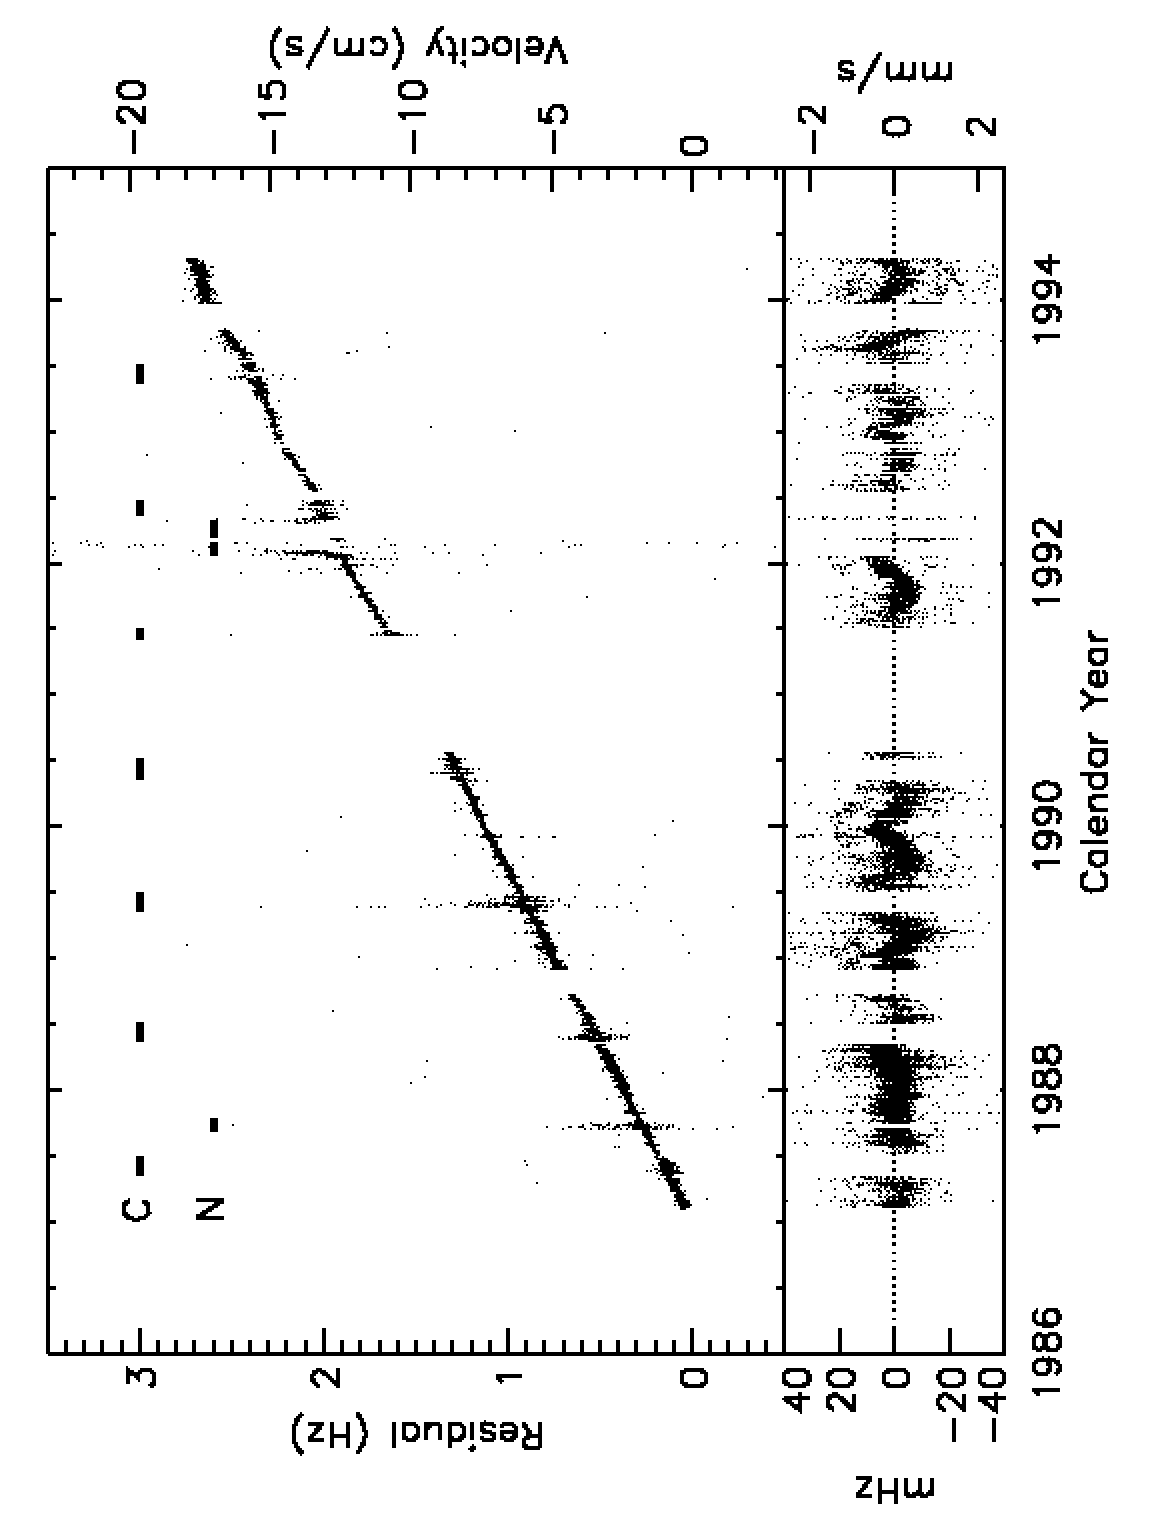
\includegraphics[angle=-90,width=0.8\linewidth]{images/M02P10beide}
\end{center}
\vskip -10pt
  \caption{Die Abweichungen von der Vorhergesagten Bahn. {\bf Oben:} ohne Berücksichtigung einer Anomalie; {\bf Unten:} mit Berücksichtigung der Anomalie. Die Beiden mit C und N markierten Zeilen oben, zeigen Zeiten an in welchen die Daten von der Auswertung ausgeschlossen wurden, weil die Daten durch Effekte Sonnen corona (C) beziehungsweise unbekannte Gründe (N) stark verrauscht waren. Es handelt bei diesem Bild um das Ergebnis von Markwardts Analyse\cite{Markwardt2002}.}\label{fig:Markwardvergl}
\end{figure} 
 
\begin{figure}[htnb]
\begin{center}
\noindent    
\psfig{figure=images/correlated,width=\linewidth,height=\textheight,keepaspectratio}
\end{center}
\vskip -10pt
  \caption{
Verlauf der anomalen Beschleunigung in Abhängigkeit von der Entfernung in Astronomischen Einheiten. Diese Tabelle zeigt das Resultat einer groben Auswertung der Daten an, sie ist noch kein Ergebnis der in Arbeit befindlichen, genauen Analyse der Daten über den gesamten Zeitraum. Die Ersterscheinung dieser Grafik konnte nicht ermittelt werden, sie taucht jedoch in zahlreichen Arbeiten auf, darunter\cite{Anderson2002}\cite{Nieto2005}\cite{Turyshev2010}
}
\label{fig:anomalie}
\end{figure} 
 
\subsection{Die Anomalie}
Geht man nun davon aus, dass unsere physikalischen Modelle richtig sind und wir alle relevanten Einflüsse berücksichtigt haben, so erwartet man im Rahmen der Messgenauigkeit für $a_P = 0$ eine Übereinstimmung im Fit.
Zunächst schien dies auch noch der Fall zu sein, nach dem Flyby-Manöver am Saturn im Jahr 1979 änderte sich dies für Pioneer 11 aber deutlich. Zu diesem Zeitpunkt befand sich die Sonde in einer Entfernung von etwa 20 AU und somit war die Beschleunigung durch den, in niedrigen Entfernungen nur ungenau berechenbaren, solaren Strahlungsdruck auf unter $5 \cdot 10^{-8} \frac{cm}{s^2}$ gesunken,
somit sank auch die Messungenauigkeit weit genug, um das nun zu Tage tretende Phänomen nicht mehr länger zu verschleiern.
Auch für Pioneer 10 stellte man bald darauf eine Abweichung fest.

Die Analyse der Daten von 1987 bis 1998 – das entspricht solaren Entfernungen von 20 bis 70 AU –
zeigte eine zeitlich konstant zunehmende anomale Blauverschiebung von
\begin{equation}
  \frac{d\Delta\nu}{dt}=(5,99\pm0,01)\cdot10^{-9}\frac{Hz}{s}
\end{equation}
wobei $\Delta\nu=[\nu_{Messung}-\nu_{Modell}]'_E$ ist\cite{Dittus2006}. Der Fehler hierbei ist nur der statistische Fehler. Die zunehmende Blauverschiebung ist im oberen Teil von Abbildung~\ref{fig:Markwardvergl} deutlich zu sehen. Lässt man die Software, die Bahn ohne eine Anomalie an die Werte fitten, so versucht sie  die Kurve durch Manöver anzupassen – man erhält dabei jedoch starke Abweichungen, weshalb ein solches Modell auszuschließen ist\cite{Markwardt2002}.

Lässt man, wie oben beschrieben, beim Fitten eine zusätzliche Beschleunigung zu, so erhält man eine wesentlich bessere Übereinstimmung (siehe Abbildung \ref{fig:Markwardvergl}, unten). Die dabei gefundenen Werte der Anomalie für die beiden Sonden sind:
\begin{eqnarray}
  a_{Pioneer 10} = (7,84\pm0,01)\cdot10^{-8}\frac{cm}{s^2} \\  
  a_{Pioneer 11} = (8,55\pm0,02)\cdot10^{-8}\frac{cm}{s^2}
\end{eqnarray}

Zwischen den obigen Werten lässt sich aus Gleichung (\ref{equ:rel}) ein direkter physikalischer Zusammenhang ableiten. Verwendet man die vereinfachte Version (\ref{equ:einf_rel}), so erhält man:
\begin{equation}
  a_{Pioneer}=\frac{dv}{dt}=\frac{1}{2}\frac{c}{\nu_E}\frac{d\Delta\nu}{dt}
\end{equation}
%oder
%\begin{equation}
%  \Delta\nu=-\nu_E \frac{2a_p t}{c}
%\end{equation}

Berücksichtigt man den Einfluss aller bekannter Effekte auf den Wert und die Unsicherheit der Größe\cite{Turyshev2004}, so erhält man einen endgültige Wert von:  
\begin{equation}
  a_{Pioneer} = (8,74\pm1,33)\cdot10^{-8}\frac{cm}{s^2}
\end{equation}

Andere Arbeiten mit den  unterschiedlichen Orbit Determination Codecs bestimmten die Beschleunigung zu $(7,70
\pm0,02)\cdot10^{-8}\frac{cm}{s^2}$ (Markwardt, 2002)\cite{Markwardt2002} beziehungsweise % anderen Wert von Markward
$(8,4\pm0,1)\cdot10^{-8}\frac{cm}{s^2}$ (Levy et al., 2008)\cite{Levy2008}.
Wobei beide Arbeiten sich nur auf Pioneer 10 beziehen und jeweils nur die statistischen Fehler angeben.
Wir wollen uns im folgenden jedoch – wie auch praktisch jede Arbeit der Fachliteratur – auf den oben angegebenen von
Anderson et al. berechneten Wert beschränken.
%% wohin damit:
% Die Standartabweichung bei einem Fit mit dieser konstanten Beschleunigung ist deutlich kleiner als ohne. % 9,8 mHz bei Levy

Der Wert mag zwar klein erscheinen, doch ist seine Größenordnung nur das $10^{-5}$ fache der Newtonschen Beschleunigung,
und er ist größer als die Faktoren $U/c^2$,$v^2/c^2$,$r a/c^2$ zur relativistischen Korrektur der newtonschen Dynamik.
% richtig?
Seit 1979 ist die Sonde um fast eine halbe Million Kilometer von der berechneten Bahn abgewichen:
\begin{equation}
  \Delta x= \frac12 \cdot a_p \cdot (2011-1979)^2 a^2\approx 445.000 km
\end{equation}

Diese Frequenzverschiebung wurde mit nur maximal 3\% Unterschied bei beiden Pioneer-Sonden unabhängig voneinander
gefunden. Das anomale Signal variiert über den analysierten Zeitraum um nur maximal 3,4\%\cite{Turyshev2004}.
Olsen zeigt jedoch, dass es bei der derzeitigen Datenlage nicht auszuschließen ist, dass die Anomalie mit der Zeit abnimmt.\cite{Olsen2006}
Die Richtung der
Beschleunigung ist mit einer Auflösung von 3° bisher noch recht ungenau bestimmt worden. Es ist daher nicht sicher möglich
zu sagen ob die Beschleunigung
in Richtung Sonne, Erde, negativer Geschwindigkeit oder Drehachse geht, dazu mehr in Kapitel \ref{fragen}.

Eine alternative Interpretation zu einer konstanten Beschleunigung, wäre eine zeitliche Beschleunigung.
So ließe sich die Anomalie auch durch eine zeitliche Beschleunigung von $a_t = (2,92 \pm 0,044) \cdot 10^{-18} s^{-2}$ schreiben.



\subsection{Variabler Teil}
Während in Normalfall die Anomalie als konstante Beschleunigung angesehen wird, wiesen betreits Anderson et al. in
ihrer Arbeit im Jahr 2002 darauf hin, dass es periodische Anteile in der Pioneeranomalie zu geben scheint. Im Jahr 2008
zeigte die „Groupe Anomalie Pioneer“ (GAP) – ein Zusammenschluss von etlichen französischen Forschungseinrichtungen –
das sich die Qualität des Fits nennenswert steigern lässt, wenn man zusätzlich zur konstanten Beschleunigung
periodische Terme verwendet.
Dabei ist es ihnen gelungen eine Beziehung zwischen dem Unterschied der Azimutalwinkel zwischen Sonde und Erde, sowie
den zeitlich veränderlichen Anteilen der Pioneeranomalie zu finden. %bäh

Die periodischen Anteile des Signals lassen sich sehr gut auf der auf Abb. FIXME dargestellten Spektralanalyse
erkennen. Die Drei großen Peaks liegen bei $f_1=0.9974\pm0.004\ Tagen$, $f_2=\frac12(0.9974\pm0.004)\ Tagen$ und 
$f_3=189\pm32\ Tagen$. Bedenkt man das 1.0 siderischer Tag = 0.9972 Tage ist, so entspricht dies genau
halbtägigen, täglichen und halbjährlichen Schwankungen. Anderson et al. ziehen dafür Messfehler – wie Fehler in den
Ephemeriden oder der Ausrichtung der Drehachse der Erde oder fehlerhafte Koordinaten der Messstationen – in Betracht.
Die Gruppe um Levey (GAP) hält dies jedoch für unwahrscheinlich, da diese Daten durch andere Beobachtungsmethoden
gestützt werden.
Sie nehmen an, dass durch eine beliebige Ursache die Ausbreitung des Tracking-Signals auf dem Weg zwischen Raumsonde und
Erde verändert wird. Sie beschreiben die Ursache als Funktion des Azimutalwinkel zwischen Sonde und Erde und fitten
dann die Fouriekoeffizienten. Dieses geometrische Modell beschreibt sowohl die täglichen, also auch die jährlichen
Schwankungen und verringert die Abweichung von den Messwerten von 9.8 mHz auf 5.5 mHz. Auch die Spektralanalyse (
Abb. FIXME) dieses fits zeigt die Verbesserung deutlich.

\bigskip

\section{Klassische Erkl\"arungen}\label{klassisch}

Bevor man neue Theorien aufstellt um diese ungew\"ohnliche
Beschleunigung zu erkl\"aren, sollte man sich zun\"achst die
klassischen Erkl\"arungen ansehen, die die Beschleunigung erkl\"aren
k\"onnten bzw. eine Fehlerabsch\"atzung der Beschleunigung geben
k\"onnen. Hierzu teilte Anderson et al. \cite{Anderson2002} die Daten von Pioneer 10 in drei Intervalle
ein, die man durch den steigenden Abstand zur Sonne und Einfl\"usse von
anderen Himmelsk\"orpern abgrenzen muss. (Abb. \ref{fig:intervalle})

\begin{figure}[htbn]
\begin{center}
\noindent    
\psfig{figure=images/intervalle,width=0.8\linewidth,height=\textheight,keepaspectratio}
\end{center}
\vskip -10pt
  \caption{Abgrenzung der drei Datenintervalle von Pioneer 10 \cite{Anderson2002}}
\label{fig:intervalle}
\end{figure} 

\subsection{Externe Fehlerquellen}\label{extern}

\subsubsection{Strahlungsdruck der Sonne}

Durch den Impuls den die Photonen des Sonnenlichts auf die Fl\"ache der Sonde
\"ubertragen entsteht eine Kraft und damit letztlich auch eine
Beschleunigung. Diese ist zwar in Flugrichtung gerichtet, muss aber
f\"ur eine Fehlerrechnung und einer genauen zuerst betrachtet werden. Ein Modell f\"ur
den Strahlungsdrucks gab es schon vor Pioneer 10 und 11. Dieses Modell
formuliert eine Beschleunigung in Abh\"angigkeit der Ausrichtung und
Entfernung der Sonde zur Sonne.

\begin{equation}\label{eins}
a_{\mathit{sd}}(r)=-\frac{\kappa f_{s}A\cos \theta
(r)}{cMr^{2}}
\end{equation}

Dabei sind:
\begin{itemize}
\item $\mathit{f_s}=1367W/(\mathit{m\cdot AU})^2$
\item $A=r^2\pi =(1,37m)^2\pi $ (als sonnenzugewandte Oberfl\"ache der Sonde wird vereinfacht
die Fl\"ache der Parabolantenne verwendet)
\item $\theta $ ist der Winkel unter dem die Photonen auf $A$ treffen. Da der Winkel immer unter 1.5° ist wird er zu $\theta = 0\degree$ vereinfacht, was lediglich zu einem Verlust an Genauigkeit von $< 4 \cdot 10^{-12} \frac{cm}{s^2}$\cite{Markwardt2002} führt.
\item $c$ ist die Lichtgeschwindigkeit
\item $M$ ist die nominelle Masse der Sonde, zum Zeitpunkt an welchem die H\"alfte des
Treibstoffs verbraucht war (F\"ur Pioneer 10 wurden 241 kg angenommen)
\item $r$ ist der Abstand Sonde-Sonne in AU
\item $\kappa $ ist der effektive Absorptions/Reflexions-Koeffizient. F\"ur
Pioneer 10 wurde ein $\kappa_0=1,71 $ ermittelt\cite{Anderson2002}.
\end{itemize}

\bigskip

So erh\"alt man bei einem Abstand von 5,2 AU eine Beschleunigung von
$-(70,0\pm 3,5)\cdot 10^{-8}\mathit{cm}/s^{2}$ mit $\kappa_{5,2 AU}=1,77$.
Da der Strahlungsdruck wie alle anderen
Gesetze im 3-dimensionalen Raum dem $1/r^{2}$ Gesetzt folgt, war die
Beschleunigung bei 10 AU noch $-18,9\cdot 10^{-8}\mathit{cm}/s^{2}$
und bei 70 AU nur noch $-0,39\cdot 10^{-8}\mathit{cm}/s^{2}$. Da der
Strahlungsdruck der Sonne sehr genau von den Auswertungsprogrammen
modelliert werden kann, liegt der Fehler f\"ur Pioneer 10 zwischen 40
und 70 AU bei $0,001\cdot 10^{-8}\mathit{cm}/s^{2}$ und f\"ur Pioneer
11 zwischen 22 und 32 AU bei $0,006\cdot 10^{-8}\mathit{cm}/s^{2}$

Da die Masse durch die Verbrennung von Treibstoff mit der Zeit auch
ver\"anderte, erh\"alt man f\"ur die Ver\"anderung von $a_{p}$ f\"ur
die 3 Intervalle\cite{Anderson2002}:

\begin{equation}
\mathit{\delta a}_{p}=[(0,040\pm 0,035),(0,029\pm 0,025),(0,020\pm
0,017)]\cdot 10^{-8}\mathit{cm}/s^{2}
\end{equation}
Man bildet das gewichtete Mittel und erh\"alt f\"ur

\begin{equation}
a_{\mathit{sd}}=(0,03\pm 0,01)\cdot 10^{-8}\mathit{cm}/s^{2}
\end{equation}

Wenn man nun f\"ur Pioneer 11 das gleiche durchf\"uhrt erh\"alt man
\begin{equation}
a_{\mathit{sd}}=(0,09\pm 0,21)\cdot 10^{-8}\mathit{cm}/s^{2}
\end{equation}

Dies kann nicht die Anomalie erkl\"aren. Ist jedoch f\"ur die
Fehlerrechnung interessant.


\bigskip

\subsubsection{Der Sonnenwind}

Der Sonnenwind beschleunigt die Pioneers \"ahnlich wie Gl. \ref{eins}, nur das
man $\frac{f_{s}}{c}$ \ durch $m_{p}v^{2}n$ ersetzt. Hier ist
$n{\approx}5/\mathit{cm}^{3}$ die Protonendichte bei 1 AU und
$v{\approx}400\mathit{km}/s$ die Windgeschwindigkeit. So erh\"alt
man\cite{Anderson2002}:
\begin{equation}
a_{\mathit{sw}}(r)=-\frac{\kappa _{\mathit{sw}}m_{p}v^{2}nA\cos \theta
}{Mr^{2}}\approx -1,11\cdot
10^{-11}(20\frac{\mathit{AU}}{r})^{2}\mathit{cm}/s^{2}
\end{equation}

Da die Protonendichte um 100\% schwanken kann, ist die tats\"achliche
Beschleunigung unvorhersehbar. Unter der konservativen
Annahme, dass diese Beschleunigung um zwei Gr\"o{\ss}enordnungen
kleiner ist als die des Strahlungsdrucks, ist sie zu vernachl\"assigenden.


\bigskip

\subsubsection{Die Effekte der Sonnencorona}

Wie in Abschnitt 3.1.2 gesehen, ist der Effekt des Sonnenwindes auf die
Beschleunigung der Sonden vernachl\"assigbar. Jedoch muss man den
Einfluss der Sonnencorona auf die Radiosignale ber\"ucksichtigen. Denn
die Elektronendichte und der Gradient der Elektronendichte beeinflussen
die Ausbreitung von Radiowellen in einem Medium. Die Zeitverz\"ogerung einer S-Band Welle auf einem Weg $l$ l\"asst sich beschreiben als
\begin{equation}
\Delta t=\frac{\pm 1}{2\mathit{cn}_{\mathit{krit}}(\nu )}\int
_{\mathit{Sonnenmittelpunkt}}^{\mathit{Sonnencorona}}n_{e}(t,r)\mathit{dl}
\end{equation}
\cite{Anderson2002}

Mit
\begin{itemize}
\item $n_{\mathit{krit}}(\nu )=1,240\cdot 10^{4}(\frac{\nu
}{1}\mathit{MHz})^{2}\frac{1}{\mathit{cm}^{3}}$ ist die kritische
Plasmadichte f\"ur eine Tr\"agerfrequenz $\nu $

\item $n_{e}(t,r)$ ist die freie Elektronendichte im Sonnenplasma
\item Das positive Vorzeichen ist f\"ur Laufzeitdaten und das negative
f\"ur Dopplerdaten
\end{itemize}

Um den Einfluss der Sonnencorona auf die Radiowellen der
Pioneer-Sonden zu verstehen, kann die Elektronendichte der Corona als
Summe einer statischen und einer ver\"anderlichen Elektronendichte
modelliert werden. Da der ver\"anderliche Teil \ kaum Einfluss auf
Dopplerdaten hat\cite{Anderson2002}, reicht es ein statisches Modell der Sonnencorona
zu betrachten. F\"ur dieses Modell erh\"alt man eine freie
Elektronendichte von\cite{Anderson2002}:

\begin{equation}
n_{e}(r,t)=A(\frac{R_{s}}{r})^{2}+B(\frac{R_{s}}{r})^{2,7}\cdot
e^{-[\frac{\Phi }{\Phi _{0}}]^{2}}+C(\frac{R_{s}}{r})^{6}
\end{equation}
Aus den Daten der Cassini-Mission wurden f\"ur die Parameter A,B und C die
folgenden Werte ermittelt:

\begin{equation*}
A=6,0\cdot 10^{3}m
\end{equation*}
\begin{equation*}
B=2,0\cdot 10^{4}m
\end{equation*}
\begin{equation*}
C=0,6\cdot 10^{6}m
\end{equation*}
Dies nennt man das {\quotedblbase}Cassini Corona Model``. Die
Auswertungsprogramme ODP/Sigma und CHASMP haben f\"ur den Fehler der Beschleunigung aufgrund der Sonnencorona den
Wert

\begin{equation}
\sigma _{\mathit{corona}}=\pm 0,02\cdot
10^{-8}\mathit{cm}/s^{2}
\end{equation}
berechnet\cite{Anderson2002}.


\bigskip

\subsubsection{Lorentzkr\"afte}

Es ist nicht unwahrscheinlich dass die Sonden eine Ladung tragen, die im
elektromagnetischen Feld des Sonnensystems einen Einfluss auf die
Geschwindigkeit hat. Die magnetische Feldst\"arke im \"au{\ss}eren
Sonnensystem liegt bei unter $10^{-5}\mathit{Gauss}$\cite{Anderson2002}.
Unter der Annahme dass die Sonden eine maximale Ladung von $0,1-1,8\mu
C$\footnote{ %% ### Fussnote nicht mehr auf zwei Seiten splitten
Ich gebe hier deshalb einen Bereich an, da die Angaben in \cite{Null1976} auf der Tatsache beruhen, dass
Pioneer 10 bei Jupiter eine magnetische Feldst\"arke von 1,135 Gau{\ss}
gemessen h\"atte. Dies ist aber laut \cite{Anderson2002}, S. 29 falsch, da f\"ur Pioneer 10 nur eine
magnetische Feldst\"arke von 0,185 Gau{\ss} gemessen wurde (Pioneer 11
ma{\ss} durch ihre gr\"o{\ss}ere Ann\"aherung 1,135 Gau{\ss}).
\begin{equation*}
B=\frac{F_{B}}{\mathit{qv}}\ \ \mathit{mit}\ \ F=m\cdot
a\ \ \mathit{ergibt}\mathit{sich}\mathit{f\text{\"u}r}\mathit{die}\mathit{Ladung}\ \ q=\frac{\mathit{ma}}{\mathit{BV}}
\end{equation*}
mit \cite{Anderson2002}, S. 29:
\begin{equation*}
\begin{gathered}v=14,36\cdot 10^{3}m/s;\ B=0,185\cdot
10^{-4}T;\ m=241\mathit{kg};\ a=20\cdot 10^{-10}m/s^{2}\end{gathered}
\end{equation*}
ergibt sich:
\begin{equation*}
q=1,8143\mu C
\end{equation*}}
tragen k\"onnen errechnet sich eine Beschleunigung von
\begin{equation}
a=\frac{\mathit{Bqv}}{M}=\frac{1\cdot 10^{-9}T\cdot 1\cdot
10^{-6}C\cdot 14,36\cdot 10^{3}m/s}{251,883\mathit{kg}}=5,7\cdot
10^{-14}m/s^{2}
\end{equation}
Mit 
\begin{itemize}
\item $B$ ist die magnetische Flussdichte
\item $q$ ist die Ladung der Sonde
\item $v$ ist die Geschwindikeit der Sonde
\end{itemize}

Diese Beschleunigung kann man vollst\"andig vernachl\"assigen.


\bigskip

\subsubsection{Die Gravitation des Kuiperg\"urtel}

Unter der Annahme, dass sich im Kuiperg\"urtel etwa 1 Erdmasse an
Partikeln befinden hat man 3 Staubverteilungen gepr\"uft: 1) eine
gleichm\"a{\ss}ige Verteilung, 2) eine 2:1 Resonanz Verteilung \ mit
einem Maximum bei 47,8 AU und 3) eine 3:2 Resonanz Verteilung mit einem
Peak bei 39,4 AU. Die letzten 2 Verteilungen wurden deswegen
ausgew\"ahlt, da diese Verh\"altnisse bei dem Resonanzeffekt von Neptun
auf Pluto beobachtet wurden. Abb.\ref{fig:kuiper} zeigt die Beschleunigung auf
Pioneer 10 von 30 bis 65 AU. Hier erkennt man eine Beschleunigung in der
Gr\"o{\ss}enordnung von $10^{-9}\mathit{cm}/s^{2}$. \ In Abb.\ref{fig:kuiper}
erkennt man zus\"atzlich, dass die Beschleunigung nicht konstant ist.
Da der Wert zwei Gr\"o{\ss}enordnungen unter der Anomalie liegt und
nicht konstant ist, kann man den Kuiperg\"urtel als Ursache der
Anomalie ausschlie{\ss}en. Infrarotmessungen von 2002 haben eine Masse
von ca. 0,3 Erdmassen im Kuiperg\"urtel entdeckt. Dies wird in der
Fehlerrechnung mit \ $\sigma _{\mathit{KG}}=\pm 3\cdot
10^{-10}\mathit{cm}/s^{2}$ ber\"ucksichtigt\cite{Anderson2002}.


\begin{figure}[htbn]
\begin{center}
\noindent    
\psfig{figure=images/kuiper,width=0.5\linewidth,height=\textheight,keepaspectratio}
\end{center}
\vskip -10pt
  \caption{Mögliche Beschleunigung der Pioneer-Sonden durch die Gravitation des Kuipergürtels \cite{Anderson2002}}
\label{fig:kuiper}
\end{figure} 


\bigskip

\subsection{Sondeninterne Fehlerquellen}\label{intern}

\subsubsection{Radiowellenr\"ucksto{\ss}}

Die Pioneer-Sonden haben eine Sendeleistung von 8 W, die wie folgt
abgestrahlt wird:
\begin{equation}
P_{\mathit{SL}}=\int _{0}^{\theta _{\mathit{max}}}\sin \theta \rho
(\theta )d\theta
\end{equation}
Dabei ist $\rho (\theta )$ die Leistungsverteilung.

Die Beschleunigung der Sonde durch die Radiowellen l\"asst sich
berechnen mit:
\begin{equation}
b_{\mathit{SL}}=\frac{\beta P_{\mathit{SL}}}{\mathit{Mc}}
\end{equation}
wobei $b_{\mathit{SL}}$ von der Erde weg zeigt. Dabei ist $\beta $ die
partielle Komponente des Strahlungsmoments, welche in entgegengesetzter
Richtung zu $a_{p}$ zeigt\cite{Anderson2002}:
\begin{equation}
\beta =\frac{1}{P_{\mathit{SL}}}\int _{0}^{\theta _{\mathit{max}}}\sin
\theta \cos \theta \rho (\theta )d\theta
\end{equation}
Messungen  zeigten\cite{Anderson2002}, dass man den Strahl als konisch annehmen kann.
Mit einem Gesamt\"offnungs\-winkel von $\theta =3,75{}^{\circ}$ ist
$\beta =0,99\pm 0,01$ und damit $w_{\mathit{SL}}=1,10\cdot
10^{-8}\mathit{cm}/s^{2}$.

Mit einem Fehler der Sendeleistung und der Ungenauigkeit der Masse
erh\"alt man als Ergebnis f\"ur die Beschleunigung der Sonden durch die
Sendeleistung
\begin{equation}
a_{\mathit{SL}}=-1,10\pm 0,11\cdot 10^{-8}\mathit{cm}/s^{2}
\end{equation}


\newpage 

\subsubsection{Ungleichm\"a{\ss}ige Abstrahlung der RTGs}

W\"ahrend dem Flug zum Jupiter war die Sonde relativ nahe an der Sonne.
Eine Erkl\"arung f\"ur die Beschleunigung k\"onnte nun folgende sein:
Die Fl\"achen der RTGs\footnote{RTG steht für radioisotope thermoelectric generator, zu Deutsch Radionuklidbatterie und ist im äußeren Planetensystem die einzig sinnvolle Energiequelle. Die Energieversorgung einer Raumsonde durch Solarzellen ist nicht praktikabel, da die Solarzellen enorme Flächen bräuchten um genug Leistung bereit zu stellen. In einem RTG zerfällt auf natürliche Weise ein $\alpha$-Strahler und erzeugt durch den Stoss der ausgesendeten Heliumkerne an anderen Atomen Wärme. Diese W\"arme nehmen thermoeletrische Bauelemente auf und wandeln sie direkt in elektrische Energie um.}, die der Sonne zugewandt waren, haben eine
h\"ohere Strahlendosis durch den Sonnenwind erfahren als die der Sonne
abgewandten. Dies geschah gleichzeitig mit dem Auftreffen von interplanetarem Staub auf die sonnenabgewandten Seiten. Dadurch entstand ein
Strahlungsgradient und somit eine ungleichm\"a{\ss}ige Abstrahlung der
RTGs. Durch die spezielle Bauweise der K\"uhlrippen aus einer
Magnesiumlegierung, die mit einem Zirkonium-Natrium Silicat beschichtet
war, besitzen die K\"uhlrippen einen hohen Emissionskoeffizienten
von ca. 0,9 und einen geringen Absorptionskoeffizienten von ca. 0,2. Um
nun $a_{p}$ hervorzurufen m\"usste es eine unterschiedliche
Abstrahlung in Front/Heck- Ausrichtung von 10\% gegeben haben. Nach
unserem Kenntnisstand des Sonnenwindes und des interplanetaren Staubs
ist es nicht m\"oglich, dass diese zwei Ph\"anomene einen derart
gro{\ss}en Gradienten mit dem richtigen Vorzeichen erzeugen k\"onnen.
Dies wurde durch visuelle Beweise der Voyager Sonden gest\"utzt\cite{Anderson2002}.

W\"ahrend den Flyby Man\"overn wurden die Sonden jedoch sehr hoher
Strahlung ausgesetzt, die eine Besch\"adigung der RTGs zur Folge haben
k\"onnte. Man h\"atte also w\"ahrend eines Flyby Man\"overs einen
Anstieg in der thermischen Emission beobachten m\"ussen. Da f\"ur die
Oberfl\"achenenergiebelastung $F\alpha T^{4}$ gilt, h\"atte man eine
Temperaturdifferenz an den K\"uhlrippen beobachten m\"ussen. Die
Durchschnittstemperatur der K\"uhlrippen lag bei ca. 440 K \cite{Anderson2002}. Um
$a_{p}$ zu erkl\"aren m\"usste ein Unterschied von 10\% bzw. $\approx$12,2 K
herrschen. Dieser Unterschied wurde jedoch nicht beobachtet und somit
kann auch dies als Ursache f\"ur die Anomalie ausgeschlossen werden. Um
diesem Effekt dennoch gerecht zu werden, wird f\"ur die Fehlerrechnung
eine unterschiedliche Abstrahlung von 1\% angenommen. Bei einer
thermischen Leistung von 2000 W liegt eine unterschiedliche Abstrahlung
von 10 W in Front/Heck-Ausrichtung vor. Da die K\"uhlrippen in einem
Abstand von 30{\textdegree} angebracht sind, ergibt sich aus
$[10W]\cdot \int _{0}^{\pi }[\sin \Phi ]d\Phi /\pi \approx
6,12W$\cite{Anderson2002} (da 4 der 12 Rippen senkrecht und parallel zur Flugrichtung
stehen) eine Ungenauigkeit von

\begin{equation}
\sigma _{\mathit{UA}}=0,85\cdot 10^{-8}\mathit{cm}/s^{2}
\end{equation}


\bigskip

\subsubsection{Aussto{\ss} von Helium aus den RTGs}

Eine weitere Erkl\"arung der anomalen Beschleunigung ist, dass durch den
$\alpha ${}-Zerfall von Pu-238 Helium aus den RTGs austritt. Die RTGs
der Pioneer Sonden wurden so konstruiert, dass das Helium aus der
Hitzequelle in den thermoelektrischen Konverter diffundieren kann. Der
Konverter ist mit einem Dichtungsring(O-Ring) abgeschlossen, der es dem Helium
allerdings erm\"oglicht in den Weltraum zu entweichen. Im gesamten Brennstoff
 der RTGs sind 5,8 kg Pu-238 enthalten\cite{Anderson2002}. Mit einer
Halbwertszeit von 87,74 Jahren werden pro Jahr ca. 0,77 g Helium mit einer
Temperatur von 433 K ausgesto{\ss}en. Dies entspricht nach $E_kin=3/2 kT$ einer
Geschwindigkeit von 1,22 km/s. Mit der Raketengleichung
\begin{equation}
a(t)=-v(t)\frac{d}{\mathit{dt}}[\ln M(t)]\ ,
\end{equation}
unser nominellen Pioneer 10 Masse von 241 kg und der Annahme, dass das
Helium die RTGs ungerichtet verl\"asst, erh\"alt man eine
Beschleunigung von $1,16\cdot 10^{-8}\mathit{cm}/s^{2}$.

Der Gasaustoss ist jedoch nicht ungerichtet, sondern, da der O-Ring an
der Seite der RTGs angebracht ist, in Richtung Sonne. Durch die
K\"uhlrippen der RTGs wird au{\ss}erdem noch Helium elastisch
reflektiert, sodass man auf eine Beschleunigung aufgrund des
Heliumaussto{\ss}es von
\begin{equation}
a_{\mathit{He}}=-(0,15\pm 0,16)\cdot 10^{-8}\mathit{cm}/s^{2}
\end{equation}
kommt\cite{Anderson2002}.


\bigskip

\subsubsection{Gasleck im Antriebssystem}

Da es keine perfekten Ventile gibt, muss man immer mit einem leichten
Gasaustritt im Antriebssystem rechnen. Einige Sonden\cite{Anderson2002} haben
deswegen Beschleunigungen von bis zu $10^{-7}\mathit{cm}/s^{2}$
erfahren. Das Antriebssystem der Pioneers besteht aus drei Paar
Korrekturd\"usen, die im 120{\textdegree} Abstand um die Parabolantenne
angebracht sind. Von diesen drei Paaren sind zwei parallel zur
Sonnenl\"angsachse ausgerichtet um die Pr\"azession der Parabolantenne
zu steuern. Ein Paar ist tangentiell zur Antenne positioniert um die
Rotation zu steuern. Aus den Ver\"anderungen der Rotationsrate in den
Intervallen i=I,II,III ist die Kraft eines Gaslecks mit einem Hebelarm
von R=1,37 m und einem Tr\"agheitsmoment von
$I_{z}=588,3\mathit{kg}\cdot\ m^{2}$
\begin{equation}
F_{\theta }=\frac{I_{z}\theta }{R}=(2,57;12,24;1,03)\cdot
10^{2}N
\end{equation}

Um nun die Kraft der zwei anderen Korrekturd\"usen abzusch\"atzen, nimmt
man an, dass diese das gleiche Gasleck haben, wie die
Rotationskorrekturd\"usen. So kann man nun annehmen\cite{Anderson2002}, dass
\begin{equation}
F_{\mathit{GL}}\simeq \pm \sqrt{(2)}F_{\theta }=(\pm 3,64;\pm
17,31;\pm 1,46)\cdot 10^{2}N
\end{equation}
ist. Unter der weiteren Annahme dass die Fehler normalverteilt sind,
liegt der Fehler f\"ur Pioneer 10 bei
\begin{equation}
\sigma _{\mathit{GL}}=\pm 0,56\cdot 10^{-8}\mathit{cm}/s^{2}
\end{equation}
Dies ist die gr\"o{\ss}te Ungenauigkeit, aber jedoch nicht gro{\ss}
genug um die Pioneer-Anomalie zu erkl\"aren.


\bigskip

\subsubsection{R\"ucksto{\ss} durch thermische Abstrahlung}\label{Hitze}

In der urspr\"unglichen Arbeit von 2002 \cite{Anderson2002} standen den Autoren nur
begrenzte Telemetriedaten zur Verf\"ugung. So haben sie einen Wert
f\"ur den R\"ucksto{\ss} der thermischen Abstrahlung und der
ungleichm\"a{\ss}igen Abk\"uhlung der Sonden von
$a_{\mathit{tA}/\mathit{Ak}}=0,55\pm 0,73\cdot
10^{-8}\mathit{cm}/s^{2}$ errechnet \cite{Anderson2002}[Tabelle X]. 2003 wurde jedoch
eine Arbeit ver\"offentlicht, die eine gerichtete thermische
Abstrahlungsleistung von 52 W angab. Dieser hohe Wert wurde durch
andere Berechnungen, wie die Annahme eines Lambertstrahlers(ca. 45 W)
oder eine Finite Elemente Methode(ca. 48 W), gest\"utzt\cite{Turyshev2010}. Diese Berechnungen zeigen, dass die Kraft der
thermischen Strahlung vollkommen untersch\"atzt wurde. Leider waren
auch die neuen Werte nur auf groben Absch\"atzungen der thermischen und
elektrischen Leistung an Board der Sonden gest\"utzt. Au{\ss}erdem
machen sie keine Aussagen \"uber den zeitlichen Verlauf der
Abstrahlung. Da f\"ur beide Pioneer Missionen mittlerweile alle
Telemetriedaten vorliegen wurden neue Untersuchungen der thermischen
Abstrahlung der Sonden durchgef\"uhrt.

Hier wurden zwei Hauptthermalquellen ausgemacht: Zum einen die RTGs und
zum anderen die elektrischen Ger\"ate an Board.


\bigskip
Da sich alle 4 RTGs einer jeden Pioneer Sonde zeitlich gleich verhalten,
kann man sie als eine Hitzequelle beschreiben. Die Leistung der RTGs
verh\"alt sich nach dem Zerfallsgesetz mit
\begin{equation}
P_{\mathit{rtg}}(t)=2^{\frac{-(t-t_{0})}{T}}P_{\mathit{rtg}}(t_{0})
\end{equation}
mit dem Zeitpunkt $t_0$ an dem die
Leistung $P_{\mathit{rtg}}(t_{0})=(650\pm 1)W/\mathit{RTG}$ gemessen
wurde und der Halbwertszeit von Pu-238 von T=87,74 a. Da man f\"ur die
abgenommene elektrische Leistung die genauen Daten kennt (Abb.\ref{fig:hitze}),
l\"asst sich die W\"armeleistung schreiben als
\begin{equation}
B_{\mathit{rtg}}(t)=P_{\mathit{rtg}}(t)-P_{\mathit{el}}(t)
\end{equation}


\bigskip

\begin{figure}[htbn]
\begin{center}
\noindent    
\psfig{figure=images/hitze,width=0.8\linewidth,height=\textheight,keepaspectratio}
\end{center}
\vskip -10pt
  \caption{Hitzeentwicklung der RTGs (rote Datenpunkte, Skala auf der linken Seite) und der elektronischen Geräte (grüne Datenpunkte, Skala auf der rechten Seite) über die Funktionsdauer von Pioneer 10 \cite{Turyshev2010}}
\label{fig:hitze}
\end{figure} 


\bigskip

In Abb. \ref{fig:hitze} ist au{\ss}erdem noch die elektrische Leistung aufgetragen,
die von ca. 160 W am Start der Mission langsam auf ca. 60 W abfiel, als
Pioneer 10 das letzte Signal sendete. Teilweise wurde die entnommene
elektrische Leistung aus den RTGs in den Ger\"aten unterschiedlich stark in Hitze umgewandelt
und abgestrahlt. Obwohl die Verteilung der Hitzequellen innerhalb der
Sonde nicht gleichm\"a{\ss}ig war, blieb die Temperaturverteilung in
der Sonde als Funktion der Zeit linear\cite{Turyshev2010}. Somit kann
man die Hitzeabstrahlung aufgrund von elektrischen Ger\"aten als eine
Hitzequelle behandeln. Die Daten hierf\"ur liefert die Telemetrie(Abb.\ref{fig:hitze}).

Die Berechnung der Kraft auf die Sonden gestaltet sich etwas einfacher,
da durch die Spinstabilisierung die Kraft \textit{F }nur entlang des
Einheitsvektors der Rotationsachse \textit{\bf s} berechnet werden muss:
\begin{equation}
F=\frac{1}{c}(\xi _{\mathit{rtg}}B_{\mathit{rtg}}+\xi
_{\mathit{el}}B_{\mathit{el}}){\bf s}
\end{equation}

Die Faktoren $\xi _{\mathit{rtg}}$ und $\xi _{\mathit{el}}$ lassen
sich aus der Geometrie und den thermischen Eigenschaften der Sonden
berechnen\cite{Turyshev2010}.

Die Berechnung dieser Kraft ist Bestandteil aktueller Studien zur
Pioneer-Anomalie. Auf jeden Fall belegen sie den vollkommen
untersch\"atzten Einfluss der thermischen Abstrahlung auf die
Beschleunigung. Mithilfe der neuen, kompletten Telemetriedaten ist es
nun m\"oglich sehr gute Finite Elemente Modelle der Pioneer Sonden im
Bezug auf die Hitzeverteilung zu erstellen. Sollte die Anomalie, wenn
auch nur teilweise, von dieser thermischen Kraft erkl\"art werden, muss
man sich erneut Gedanken \"uber die Konstanz von $a_{p}$ machen.


\bigskip

\subsection{Fehlertabelle und endg\"ultiges Ergebnis}

In Kapitel \ref{extern} und \ref{intern} haben wir gesehen, dass die meisten Effekte, die 
die Pioneer Sonden erfahren, nur zu einem sehr kleinen Teil Einfluss auf die
Beschleunigung haben. Wir haben in dieser Arbeit nur die wichtigsten
Fehlerquellen zusammengefasst. Diese und andere Fehlerquellen, ihre
Werte und Ungenauigkeiten sind in nachfolgender Tabelle aufgelistet.


\bigskip
\begin{table}[htbn]\label{fehler}
\tablesize
\newcommand{\mc}[3]{\multicolumn{#1}{#2}{#3}}
\centering
\begin{tabular}{|p{\tablewidth}|c|c|}
\hline
Beschreibung &
Wert $\cdot (10^{-8}) cm/s^2$ &
$\sigma\ in\ (10^{-8}) cm/s^2$\\ \hline
\mc{3}{|c|}{\bf 1. Externe Fehlerquellen} \\ \hline
Strahlungsdruck der Sonne &
\raggedleft -0,03 &
 0,01\\ \hline
Sonnenwind &
~
 &
 {\textless}10\^{}-3\\ \hline
Sonnencorona &
~
 &
 0,02\\ \hline
Elektromagnetische Lorentzkr\"afte &
~
 &
 {\textless}10\^{}-4\\ \hline
Einfluss der Gravitation des Kuiperg\"urtel &
~
 &
 0,03\\ \hline
Einfluss der Erdorientierung &
~
 &
 0,001\\ \hline
Mechanische und Phasenstabilit\"at der DSN Antennen &
~
 &
 {\textless}0,001\\ \hline
Phasenstabilit\"at und Uhren &
~
 &
 {\textless}0,001\\ \hline
DSN Antennen Orte &
~
 &
 {\textless}10\^{}-5\\ \hline
Troposph\"are und Ionosph\"are &
~
 &
 {\textless}0,001\\ \hline
\mc{3}{|c|}{\bf 2. Sonden interne Fehlerquellen}\\ \hline
R\"ucksto{\ss} der Radiowellen &
\raggedleft -1,1 &
 0,11\\ \hline
Hitze, reflektiert von der Sonde &
\raggedleft {}0,55 &
 0,55\\ \hline
Ungleichm\"a{\ss}ige Hitzeabstrahlung der RTGs &
~
 &
 0,85\\ \hline
Ungleichm\"a{\ss}ige Abk\"uhlung der Sonden &
~
 &
 0,48\\ \hline
Heliumaussto{\ss} aus den RTGs &
\raggedleft -0,15 &
 0,16\\ \hline
Gaslecks &
~
 &
 0,56\\ \hline
Unterschiede zwischen den Sonden &
\raggedleft -0,17 &
 0,17\\ \hline
\mc{3}{|c|}{\bf 3. Rechnerische Fehlerquellen}\\ \hline
Numerische Stabilit\"at der Finite Elemente Methode &
~
 &
 0,02\\ \hline
Genauigkeit der Fehlerabsch\"atzung und Modelle &
~
 &
 0,13\\ \hline
Mismodellierung von Man\"overn &
~
 &
 0,01\\ \hline
Mismodellierung der Sonnencorona &
~
 &
 0,02\\ \hline
Jahres- und Tagesschwankungen &
~
 &
 0,32\\ \hline
\end{tabular}
\caption{Fehlertabelle}
\label{tab:fehler}
\end{table}

\noindent Das Ergebnis der anormalen Beschleunigung von Pioneer 10 und 11 liegt
bei\cite{Anderson2002}
\begin{equation}
a_{p(\mathit{gemessen})}=(7,84\pm 0,01)\cdot
10^{-8}\mathit{cm}/s^{2}\ .
\end{equation}
Bezieht man nun die Werte der Fehler und deren Ungenauigkeit von Kapitel
\ref{extern} und \ref{intern} mit ein, so erh\"alt man mit den Werten der Fehlertabelle
und mit
\begin{equation}
a_{p}=a_{p(\mathit{gemessen})}-(w_{p}\pm \sigma _{p}) \ ,
\end{equation}
wobei $w_{p}$ der Wert und $\sigma _{p}$ die jeweilige Ungenauigkeit
ist, den bekannten Wert f\"ur $a_{p}=(8,74\pm 1,33)\cdot
10^{-8}m/s^{2}$.

\FloatBarrier
\section{ Dunkle Materie}\label{Dm}

Nachdem die Pioneer-Anomalie entdeckt wurde, kamen erste Theorien auf,
dass die Anomalie ein Indiz f\"ur Dunkle Materie in unserem
Sonnensystem sein k\"onnte. Verschiedene Verteilungen der Dunklen
Materie wurden durchgerechnet und so kann zum Beispiel eine Scheibe mit
einer Dichte von etwa $4\cdot 10^{-16}\mathit{kg}/m^{3}$ im
\"au{\ss}eren Sonnensystem die Anomalie erkl\"aren. Allerdings d\"urfte
diese Dunkle Materie nicht wie leuchtende Materie gravitativ
beeinflussbar sein\cite{Turyshev2010}. Sprich, diese Scheibe wird nicht
von Planeten beeinflusst und somit nicht angeh\"auft. Dies ist jedoch
unwahrscheinlich. Wenn die Pioneer-Anomalie einen gravitativen Ursprung
h\"atte, so m\"usste sie nach Newton mit $1/r^{2}$ abnehmen. Eine
derartige Abnahme h\"atte man in den 2002 vorliegenden Datenintervallen
beobachten m\"ussen, was aber nicht geschehen ist. Ein weiteres
Argument gegen die Dunkle Materie als Grund f\"ur die Pioneer-Anomalie
ist die Masse und Dichte von Dunkler Materie, die n\"otig w\"aren um
den Effekt zu verursachen. Es w\"are in einem Abstand von 50 AU eine
Masse von mindestens $3\cdot 10^{-4}$ Sonnenmassen (sprich
$5,967\cdot 10^{26}\mathit{kg}$) mit einer Dichte von $6,0\cdot
10^{18}\mathit{kg}/\mathit{AU}^{3}$ n\"otig. Xu et al. \cite{Xu2008} argumentieren jedoch, dass \"uber die gesamte Lebensdauer
von unserem Sonnensystem von $4,5\cdot 10^{9}a$ sich maximal eine Dichte von
$2,0\cdot 10^{17}\mathit{kg}/\mathit{AU}^{3}$ h\"atte ansammeln
k\"onnen. Au{\ss}erdem sei die Masse an Dunkler Materie im gesamten
Sonnensystem nur ca. {}10\textsuperscript{20 }kg, womit die
Pioneer-Anomalie in keiner Weise erkl\"art w\"are.



\section{Dunkle Energie}\label{De}



Schon fr\"uh fiel auf, dass f\"ur den Wert der Pioneer-Anomalie
$a_{p}\simeq \mathit{cH}_{0}$ gilt, wenn c die
Vakuumlichtgeschwindigkeit und $H_0$ die
derzeitige Hubble-Konstante ist. Deshalb wurden Vermutungen
laut, dass die Anomalie mit der Ausdehnung des Universums und somit mit
der Dunklen Energie in Zusammenhang steht\cite{Turyshev2010}. Die Idee hierzu ist,
dass die Anomalie gar keine echte Beschleunigung ist, sondern nur das
Doppler-Signal durch die Ausdehnung des Universums beeinflusst wird.
Die Grundfrage hier war also ob die Dunkle Energie einen messbaren
Einfluss auf elektromagnetische Wellen hat.



Die Sonde bewegt sich mit der Geschwindigkeit $v$. Demnach w\"are
die Beschleunigung durch das sich ausdehnende Universum $a_H$:

\begin{equation*}
a_{H}=v\cdot H_{0}=\frac{v}{c}\cdot c\cdot H_{0}
\end{equation*}

Man sieht deutlich, dass die Beschleunigung
$a_H$ um den Faktor v/c kleiner w\"are,
als die beobachtete $a_p$
Au{\ss}erdem ist $c\cdot H_{0}$ f\"ur
$H_{0}=73,2\frac{\mathit{km}}{s\cdot \mathit{Mpc}}$ nur eine
Ann\"aherung an den tats\"achlichen Wert der Anomalie. Um den exakten
Wert f\"ur $a_p$ zu erhalten br\"auchte
man eine Hubble-Konstante mit einem Wert von $H_{0}=95\pm
14\frac{\mathit{km}}{s\cdot \mathit{Mpc}}$, was weit außerhalb des Fehlerbereichs von $H_0$ liegt. Ein weiteres
Argument gegen den Einfluss der Dunklen Energie ist, dass die
Beschleunigung in Richtung Sonne zeigt. W\"are die Dunkle Energie
tats\"achlich die Ursache, w\"urden die Pioneer-Sonden von der Sonne
bzw. der Erde weg beschleunigt. Im Doppler-Signal w\"urde sich das in
einer Rotverschiebung, anstatt in der beobachteten
Blauverschiebung \"au{\ss}ern.




\bigskip
\section{Modifizierte Newtonsche Mechanik (MOND)}

Die modifizierte newtonsche Mechanik (MOND) wurde Mitte der 1980er Jahre
von Mordehai \ Milgrom als Gegenentwurf zur dunklen Materie entwickelt.
Ihre ursprüngliche Motivation ist es die gemessene abflachende
Rotationskurve von Galaxien zu erklären, die sich deutlich von der
Kurve unterscheidet, die nach den keplerschen Gesetzten berechnet
wurde. Das soll erreicht werden indem das zweite newtonsche Gesetz bzw.
das Gravitationsgesetz modifiziert wird. 


\bigskip

Das zweite newtonsche Axiom besagt, dass eine Masse m an der eine Kraft
F anliegt die Beschleunigung a erfährt: 

\begin{equation*}
F=m\cdot a
\end{equation*}
Dieser Zusammenhang kann allerdings für sehr kleine Beschleunigungen nur
sehr schwer bis gar nicht experimentell überprüft und nachgewiesen
werden. In Galaxien bewirkt die Schwerkraft der Sterne aber nur solche
kleinen Beschleunigungen, da sie sehr weit voneinander entfernt sind.
Milgroms Idee \cite{Bekenstein1984} war es daher das zweite newtonsche Gesetz für sehr
kleine Beschleunigungen abzuwandeln in

\begin{equation*}
F=m\cdot a\cdot \mu (a/a_{0})
\end{equation*}
 $a_{0}$ ist eine neue Naturkonstante, die angibt ab welchen
Beschleunigungen die Modifikation wirksam wird. Milgrom bestimmte sie
aus den Messungen der Rotationsgeschwindigkeiten möglichst vieler
Galaxien als ungefähr

\begin{equation*}
a_{0}=2\cdot 10^{-10}\frac{m}{s^{2}}
\end{equation*}
 $\mu (x)$ ist eine unspezifizierte Funktion welche folgende Bedingungen
erfüllt:

\begin{itemize}
\item  $\mu (x\gg 1)\approx 1$, so dass für große Beschleunigungen die
newtonsche Mechanik gilt
\item $\mu (x\ll 1)\approx x$
\end{itemize}
In der Literatur sind für  $\mu (x)$ am häufigsten verwendeten
Funktionen:

{\centering  $\mu (x)=\frac{x}{1+x}$ $\mu
(x)=\frac{x}{\sqrt{1+x^{2}}}$\par}

Will man jetzt MOND in Hinblick auf die Pioneer Anomalie \cite{Turyshev2010}
überprüfen, muss man als erstes betrachten, welche Auswirkungen die
Theorie auf die Zentripetalbeschleunigung  $a_{z}$ einer Masse m hat,
die sich im Gravitationsfeld eines Körpers der Masse M befindet.

Nach Newton gilt mit der Gravitationskonstante G:

{\centering  $F_{g}=\frac{G\cdot {M\cdot m}}{r^{2}}$\par}

Damit gilt für  $a_{z}$

\begin{equation*}
a_{z}=\frac{v^{2}}{r}=\frac{G\cdot {M}}{r^{2}}
\end{equation*}
Löst man diese Gleichung nach  $v^{2}$ auf, so erhält man:

\begin{equation*}
v^{2}=\frac{G\cdot M}{r}
\end{equation*}
Nach MOND gilt für sehr kleine Beschleunigungen:

\begin{equation*}
a_{z}\mu (\frac{a_{z}}{a_{0}})=\frac{G\cdot {M}}{r^{2}}
\end{equation*}
Da  $\frac{a_{z}}{a_{0}}\ll 1$ gilt  $\mu
(\frac{a_{z}}{a_{0}})=\frac{a_{z}}{a_{0}}$

Setzt man dies nun in die obige Gleichung ein und löst nach  $a_{z}$
auf, so erhält man:

\begin{equation*}
a_{z}=\frac{\sqrt{M\cdot G\cdot a_{0}}}{r}
\end{equation*}
Mit  $a_{z}=\frac{v^{2}}{r}$ erhält man hier für  $v^{2}$

\begin{equation*}
v^{2}=\sqrt{M\cdot G\cdot a_{0}}
\end{equation*}
Zusammenfassend gilt also nach der modifizierten newtonschen Dynamik:

\begin{itemize}
\item  $v^{2}=\frac{G\cdot M}{r}$ für  $a_{z}\gg a_{0}$ oder kleine
Abstände
\item  $v^{2}=\sqrt{M\cdot G\cdot a_{0}}$ für  $a_{z}\ll a_{0}$ oder
große Abstände
\end{itemize}
Betrachtet man nun die Pioneer Anomalie, kann man davon ausgehen, dass 
$a_{0}\ll \frac{G\cdot M}{r}$.

Wählt man nun  $\mu (x)=1+\frac{\zeta }{x}$ bekommt man für  $a_{z}$
folgendes Ergebnis:

\begin{equation*}
a_{z}=-\ \frac{G\cdot M}{r^{2}}-\zeta \cdot a_{0}
\end{equation*}
Für  $\zeta =7$ ist 

\begin{equation*}
\zeta \cdot a_{0}=8,4\cdot 10^{8}\frac{\mathit{cm}}{s^{2}}
\end{equation*}
was der anomalen Beschleunigung der Pioneer-Sonden entspricht.

\bigskip

\section{Zukünftige Forschung}

\subsection{Offene Fragen}

Obwohl die anomale Beschleunigung der Raumsonden Pioneer 10 und 11
bereits seit Anfang der 1980-er Jahre bekannt ist, gibt es noch viele
unbeantwortete Fragen\cite{Turyshev2010}. Sie und vor allem die fehlenden Antworten
k\"onnen wichtige Hinweise auf den wahren physikalischen Hintergrund
der Anomalie liefern.


\bigskip

Ein wichtiger Punkt ist, dass die exakte Richtung des
Beschleunigungsvektors immer noch unklar ist. Der Wert  $a_{p}=(8.74\pm
1.33)\times 10^{-8}\frac{\mathit{cm}}{s^{2}}$ wurde unter der Annahme
berechnet, dass die Beschleunigung in Richtung Sonne zeigt. Wegen
Unsicherheiten in der Doppler Navigation kann die Richtung der Anomalie
nur bis auf einen \"Offnungswinkel von 3{\textordmasculine} genau
bestimmt werden. Aufgrund der gro{\ss}en Entfernung der Sonden l\"asst
diese Ungenauigkeit insbesondere vier verschieden M\"oglichkeiten zu,
welche jeweils auf eine andere Ursache hinweisen.


\begin{figure}[htbn]
\begin{center}
\noindent    
\psfig{figure=images/richtung,width=\linewidth,height=\textheight,keepaspectratio}
\end{center}
\vskip -10pt
  \caption{Die möglichen Richtungen der Pioneer-Anomalie (1) Richtung Sonne (2) Richtung Erde (3) entlang des Geschwindigkeitsvektors (4) entlang der Spin-Achse\cite{Turyshev2010}}
\label{fig:flugbahn}
\end{figure} 

\bigskip

Falls die Sonden tats\"achlich in Richtung der Sonne beschleunigt werden
sollten, w\"are es ein Hinweis darauf, dass die Anomalie von einer
Kraft herr\"uhrt, die von dort Ausgeht. Da die Gravitation als Kraft in
Frage k\"ame, k\"onnte es ein Anzeichen daf\"ur sein, das eine
Modifikation das entsprechenden physikalischen Gesetzes notwendig
w\"are.


\bigskip

Die zweite M\"oglichkeit ist, dass die Beschleunigung in Richtung Erde
zeigt. Eine wahrscheinliche Ursache w\"aren hier die
Ausrichtungsman\"over der Sonden, wie zum Beispiel nach dem Vorbeiflug
an einem Planeten. Bei dieser Konstellation k\"onnte der Fehler aber
auch in der Hardware der DSN-Antennen oder der Signal\"ubertragung
liegen.


\bigskip

Es kommt noch in Frage, dass die Beschleunigung die Richtung des
Geschwindigkeitsvektors zeigt. Das k\"onnte darauf hindeuten, das die
Beschleunigung ihren Ursprung in einer Kraft hat, die von der
Tr\"agheit der Sonden ausgeht. Des Weiteren k\"onnten die Sonden bei
diesem Szenario durch Reibung, zum Beispiel durch Staub, abgebremst
werden.


\bigskip

Als Viertes bleibt noch die Richtung der Spin-Achse. Das w\"urde den
Versuch unterst\"utzen die Erkl\"arung f\"ur die Anomalie innerhalb der
Sonden zu finden. Korrekterweise sollte deshalb also von einer
Beschleunigung in Richtung des inneren Bereiches des Sonnensystems
gesprochen werden.


\bigskip

Das zu Stande kommen die Pioneer-Anomalie zum Beispiel durch
Hitzeabstrahlung der Sonden k\"onnte als Ursache komplett
ausgeschlossen werden, wenn man mit Sicherheit w\"usste, dass die
Beschleunigung \"uber einen sehr langen Zeitraum hin konstant ist.
\"Uber das Langzeitverhalten der Anomalie ist allerdings bis jetzt noch
zu wenig bekannt. Es ist, nach heutigem Kenntnisstand, durchaus
denkbar, dass die Anomalie nach einer gewissen Zeit wieder komplett
verschwindet, oder aber noch weiter w\"achst.


\bigskip

Diese \"Uberlegungen f\"uhren direkt zu den n\"achsten Fragen, deren
Beantwortung noch einiges Licht ins Dunkel bringen kann. In welchen
Distanzen genau kann diese Beschleunigung beobachtet werden? Die Daten
von Pioneer 10 und 11 best\"atigen ihre Existenz in einer Entfernung
von ungef\"ahr 20 - 70 AU. Doch was passiert au{\ss}erhalb dieses
Bereichs? Kann die Anomalie auch in der N\"ahe der Sonne beobachtet
werden? 

Die Flugbahnen beider Sonden lagen, um die Planeten zu besuchen, in der
Ekliptik. Wirkt sie sich auch auf Sonden aus, die sich senkrecht zur
Ekliptik bewegen?


\subsection{Neue Analyse aller Vorhandener Daten}
Die Analyse von Anderson et al., 2002 betrachtete nur die Pioneer 10-Daten in der Zeit vom 3. Januar 1987 bis zum 22.
July 1998 (40 AU bis 70,5 AU) und die Pioneer 11-Daten vom 5. Januar 1987 bis zum 1. Oktober 1990 (22,4 AU bis 31,7
AU). Jedoch empfing man bis zum 27. April 2002 brauchbare Daten von Pioneer 10. (Die Daten von Pioneer 11 waren ab
Oktober 1990 nicht mehr brauchbar) Auch die anderen erwähnten Analysen bezogen sich immer auf etwa den selben Zeitraum.

Die Daten von Pioneer 10 aus dem Zeitraum von 1998 bis 2002 wurden also noch nicht untersucht. Noch
Erfolgversprechender wäre jedoch eine Analyse der frühen Daten. Die Anomalie wurde bereits ab 1979 beobachtet und durch
bessere Berechnung des solaren Strahlungsdruck könnten auch die noch früheren Daten wichtige Informationen liefern. Ees
ist daher geplant die kompletten Daten, vom Start der Sonden, bis zu den letzten verwertbaren Signalen neu zu
analysieren.

% Es ist geplant am ZARM in Zusammenarbeit mit dem JPL die gesammten Pioneer Daten vom Start bis zum letzten Signal neu
% zu analysieren	% aus Physikjournal

% Wohin mit ``bei 20 AU (~1980) sinkt der solare Strahlungsdruck auf unter 5*10^-8 cm/s^2''?

\bigskip
…
\bigskip



\subsection{Zuk\"unftige Missionen}

Die Analyse des gesamten Datensatzes der beiden Pioneer-Sonden bringt
Klarheit bei Fra\-gen wie, ob die Anomalie auch schon in Erd- oder
Sonnenn\"ahe festgestellt werden kann. Andere R\"atsel k\"onnen nicht
so leicht gel\"ost werden. Um zum Beispiel die Richtung des
Be\-schleunigungsvektors exakt festzustellen oder zu ermitteln in
welchem Bereich genau die Anomalie auftritt, wird eine neue Mission
ben\"otigt. An sie werden bestimmte Anforderun\-gen gestellt\cite{alle2005}\cite{Nieto2004b}\cite{Turyshev2004b}\cite{Nieto2004},
 um den Wert der Beschleunigung genau zu bestimmen
und m\"ogliche Fehlerquellen genau identifizieren und ausschlie{\ss}en
zu k\"onnen.


\bigskip

Das wissenschaftliche Ziel dieser Mission wird sein, die
Pioneer-Anomalie zu best\"atigen und so genau wie m\"oglich zu
erforschen. Ihr Wert soll bis auf mindestens 
$10^{-10}\mathit{cm}/s^{2}$ ge\-nau gemessen werden. Es ist
erforderlich eine h\"ohere r\"aumliche und zeitliche Aufl\"osung der
Beschleunigung zu erreichen, um genauere Aussagen \"uber ihre Richtung
und ihren zeitlichen Verlauf machen zu k\"onnen. Interne und externe
Fehlerquellen m\"ussen hierzu genau gepr\"uft und gemessen werden. Es
geh\"ort also auch dazu, dass der Strahlungsdruck der Sonne gemessen
wird und die elektrische Ladung, die sich auf der Oberfl\"ache der
Son\-de ansammelt. Auf der Mission sollen au{\ss}erdem noch
verschiedene Erkl\"arungsmodelle ge\-testet und die Ursache der
Anomalie gefunden werden. Deshalb wird es n\"otig sein das newtonsche
Gravitationspotential in gro{\ss}en Entfernungen genau zu bestimmen und
die Bedingungen im tiefen Weltraum zu erforschen. Eine weitere Option
ist noch die Sonde auf eine Bahn senkrecht zur Ekliptik zu bringen, um
zu \"uberpr\"ufen, wie sich die Anomalie dort verh\"alt.


\bigskip

Um eine Empfindlichkeit f\"ur die Beschleunigungsmessung in Richtung
aller 3 Achsen der Sonde von ca.  $10^{-10}\mathit{cm}/s^{2}$ zu
erreichen, ist eine Navigation n\"otig, die pr\"aziser ist, als die der
Pioneers. Daf\"ur ist eine spin-stabilisierte Sonde vorteilhaft. Im
Gegensatz zur 3-Achsen Stabilisation, bereitet das Austreten von
Treibstoff bei der Navigation von spin-stabilisier\-ten Objekten kaum
Probleme. Au{\ss}erdem sind weniger Man\"over zur Korrektur der Lage
notwendig. Bei solchen Ma{\ss}nahmen kann es n\"amlich sein, dass
ungewollt Treibstoff aus\-tritt, was ihre Berechnung enorm erschwert.


\bigskip

Aus den oben genannten Gr\"unden braucht man Korrekturd\"usen,
Kraftstoffleitungen und eine Treibstoffanzeige, die sehr pr\"azise
kalibriert sind, und zus\"atzlich noch genaue Kennt\-nisse \"uber die
zeitliche Entwicklung des Treibstoffverbrauchs. Da diese Informationen
be\-sonders wichtig sind, um die Flugbahn der Sonde m\"oglichst genau
zu bestimmen, werden Sensoren ben\"otigt, die \"uber eine lange Zeit
Daten mit der geforderten Genauigkeit liefern. In diesem Bereich muss
aber noch einiges an Entwicklungsarbeit geleistet werden, da die
Sensoren, die zur Zeit erh\"altlich sind, nicht exakt genug arbeiten
und zu schnell verschlei\-{\ss}en. Eine Echtzeit Anzeige und Kontrolle
ihrer Leistung w\"are au{\ss}erdem noch erw\"unscht.


\bigskip

Die Sonde soll \"ahnlich navigiert werden wie die beiden Pioneer-Sonden,
\"uber Entfernungs- und Geschwindigkeitsbestimmung mit Hilfe von
Radiowellen. Die Entfernung wird \"uber die Laufzeit und die
Geschwindigkeit \"uber die Dopplerverschiebung des Signals ermittelt.
Bei der neuen Mission wird dazu aber nicht nur ein Frequenzband
verwendet, sondern es wird das {\quotedblbase}Dual Band Tracking``
angewendet, welches, wie der Name schon sagt, zwei Fre\-quenzb\"ander
benutzt. Das X-Band (8 -- 12 GHz) und das Ka-Band (26,5 -- 40 GHz) sind
hierf\"ur vorgesehen. Nach M\"oglichkeit sollen noch das
VLBI\footnote{Beim VLBI-Verfahren\cite{vlbi}, wird das selbe Radiosignal
von mehreren, weit auseinander stehenden Antennen empfangen.Die Daten
von den einzelnen Antennen werden zusammen mit einer einheitlichen
Zeitinformation gespeichert. Sp\"ater werden die Daten und
zugeh\"origen Zeiten der verschiedenen Antennen verglichen. So erh\"alt
man den den Laufzeitunterschied des Signals zu den Antennen und kann
daraus die Entfernung des Senders bestimmen. Da die Antennen, wegen der
Speicherung der Daten, nicht mit einem Kabel verbunden sein m\"ussen,
k\"onnen sie sehr weit weg voneinander aufgestellt werden, was das
Aufl\"osungsverm\"ogen des Verfahrens deutlich erh\"oht.}{}- (Very Long
Baseline Interfe\-rometry) und/oder das $\Delta
$DOR-Verfahren\footnote{Das $\Delta $DOR-Verfahren\cite{delta} funktioniert
so \"ahnlich wie das VLBI. Auch hier wird der Laufzeitunterschied eines
Signals zu zwei weit auseinander stehenden Antennen ermittelt. Dieses
Signal wird dann aber noch mit dem eines Quasars in der N\"ahe der
Sonde abgeglichen, dass einen vergleichbaren Weg zur\"uckgelegt hat.
Die Position des Quasars ist durch vorherige Messungen sehr genau
bekannt. So k\"onnen Fehler, die durch verschiedene St\"orfaktoren, wie
den Sonnenwind oder die Erdatmosph\"are, entstehen, genau ermittelt und
eliminiert werden.} (Delta Differential One-way Ranging) hinzu kommen.
Damit w\"are dann eine genaue Winkelbestimmung m\"oglich, die
ben\"otigt wird um die drei-dimensionalen Beschleunigungsdaten richtig
zu rekonstruieren. 


\bigskip

Nat\"urlich muss die Sonde eine interne Energieversorgung haben. Da
diese Mission in den tiefen Weltraum und somit weit weg von der Sonne
f\"uhrt, kommen Solarzellen nicht in\-frage. Noch heute gibt es f\"ur
dieses Problem keine andere L\"osung, als die schon bei den
Pioneer-Sonden verwendeten RTGs. Denn nur diese k\"onnen zuverl\"assig
Energie \"uber einen langen Zeitraum liefern.


\bigskip

Die Platzierung der RTGs stellt eine gro{\ss}e Herausforderung dar, denn
sie emittieren enorm viel Hitze. Um das als Ursache f\"ur die Anomalie
ausschlie{\ss}en zu k\"onnen, sollte die Abstrahlung m\"oglichst
symmetrisch sein. Die RTGs sind aber nicht die einzige W\"arme\-quelle
der Sonde. Auch die Korrekturd\"usen, die verbaute Elektronik und viele
andere Bestandteile emittieren W\"armestrahlung. Diese m\"usste f\"ur
jedes einzelne Bauteil so genau wie m\"oglich untersucht werden.
Seitlich soll die Strahlung durch Abdeckungen abge\-schirmt werden, so
dass sie nur nach vorne oder hinten entweichen kann und ihr
R\"ucksto{\ss} nur in oder gegen die Flugrichtung wirkt. Dies alles
hilft den drei-dimensionalen Vektor des thermischen R\"ucksto{\ss}es
sehr exakt zu ermitteln. Dazu tragen aber auch noch alle
reflektierenden Oberfl\"achen der Sonde bei. Deshalb m\"ussten diese
aus Materialien beste\-hen, bei denen vor allem der Alterungsprozess
und die Abstrahleigenschaften sehr genau bekannt sind. Im Idealfall
soll die Sonde so ausbalanciert und symmetrisch konstruiert werden,
dass alle solchen thermischen Einfl\"usse verschwinden.


\bigskip

Eine Neuerung gegen\"uber den Pioneer-Sonden wird sein, dass man an der
neuen Kon\-struktion zwei identische, gegen\"uberliegende Antennen
anbringen wird, die das Radiosi\-gnal gleichzeitig zur Erde und die
entgegengesetzte Richtung absenden. So bleibt die Son\-de in ihrem
Aufbau symmetrisch. Der R\"ucksto{\ss} durch das Senden des Signals
hebt sich auf und muss in der Berechnung nicht mehr ber\"ucksichtigt
werden. Die wichtigste Funktion der Antennen wird aber sein,
zweifelsfrei zu ermitteln ob es sich bei der Anomalie um einen externen
oder internen Effekt handelt. Nachdem pr\"azise Daten der Anomalie mit
einer Orientierung der Antennen aufgenommen wurden, etwa ein bis zwei
Jahre lang, wird die Sonde mit Hilfe von Lichtsensoren, die sich an der
Sonne oder bestimmten Sternen orientieren, um 180{\textdegree} gedreht.
Nun sendet die Antenne, die zuvor nach au{\ss}en gerichtet war, Daten
zur Erde und umgekehrt. Anschlie{\ss}end werden wieder ein bin zwei
Jahre lang pr\"azise Daten aufgenommen und diese dann mit denen der
anderen Antenne verglichen. Stellt man keine Ver\"anderung fest,
best\"atigt dies einen sondenexternen Effekt, \ \"andert sich aber das
Vorzeichen, ist die Ursache sondenintern. Jedes andere Ergebnis, das
von Null verschieden ist, zeigt, dass sowohl ein interner als auch ein
externer Effekt eine Rolle spielen. Ersterer hat dann eine Gr\"o{\ss}e
der H\"alfte der Differenz der beiden Messungen und Letzterer der
H\"alfte der Summe. 


\begin{figure}[htbn]
\begin{center}
\noindent    
\psfig{figure=images/yoyoside,width=0.5\linewidth,height=\textheight,keepaspectratio}
\end{center}
\vskip -10pt
  \caption{Seitenansicht der "Yo-Yo"-Sonde\cite{Nieto2004}}
\label{fig:yoyoside}
\end{figure} 

\begin{figure}[htbn]
\begin{center}
\noindent    
\psfig{figure=images/yoyotop,width=0.5\linewidth,height=\textheight,keepaspectratio}
\end{center}
\vskip -10pt
  \caption{Aufsicht der "Yo-Yo"-Sonde\cite{Nieto2004}}
\label{fig:yoyotop}
\end{figure} 


Um das aber tats\"achlich genau so rechnen zu k\"onnen, braucht man
eine komplett symmetrische Sonde wie sie im
{\quotedblbase}Yo-Yo``-Aufbau vorgeschlagen wird. Das Bild zeigt diesen
Aufbau von oben (links) und von der Seite (rechts) in verschiedenen
Ma{\ss}st\"aben. An den beiden langen Auslegern, die in der Draufsicht
gut zu erkennen sind, sollen die RGTs ange\-bracht werden. Sie sollen
eine L\"ange von 2 -- 2,5 m haben. Je nach dem wie die Mission
endg\"ultig gestaltet wird, kann man an dem dritten Ausleger ein
Instrumentenpaket an\-bringen, um die interstellare Materie
au{\ss}erhalb des Sonnensystems zu erforschen. Zur rei\-nen
Untersuchung der Pioneer-Anomalie, kann man dort auch noch ein drittes
RTG befestigen, was erheblich zur Symmetrie der Sonde beitragen
w\"urde. In der Seitenansicht sind die oben beschriebenen
W\"armeabdeckungen und die Antennen zu sehen. Als Vorlage f\"ur
Letztere wurde die Cassegrain Antenne der Sonde Cassini angepasst.


\bigskip

Eine interessante Modifikation des Aufbaus ist, dass man anstelle der
zweiten Antenne an der Erdabgewandten Seite eine kleine Probemasse
befestigt. Bringt man diese in einem Abstand von {\textgreater} 250 m
von der Sonde an, kann man mit ihrer Hilfe noch eine zweite
Best\"a\-tigung f\"ur die Anomalie erhalten. Die Sonde selbst wird
durch die oben beschriebenen Ra\-diosignale navigiert. Die Bewegung der
Testmasse relativ zur Sonde wird mit Laser-Ab\-standsmessung bestimmt.
Auf diese Weise l\"asst sich die Pioneer-Anomalie zus\"atzlich noch mit
einer zweiten Methode \"uberpr\"ufen. 


\begin{figure}[htbn]
\begin{center}
\noindent    
\psfig{figure=images/lasersonde,width=\linewidth,height=\textheight,keepaspectratio}
\end{center}
\vskip -10pt
  \caption{\cite{alle2005}}
\label{fig:lasersonde}
\end{figure} 

\bigskip

Bei gro{\ss}en Himmelsk\"orpern mit gebundenen und nur wenig
exzentrischen Bahnen konnte die Anomalie nicht festgestellt werden und
bei den Pioneer-Sonden wurde sie erst ent\-deckt, als sie sich auf
ihrer hyperbolischen Bahn befanden um das Sonnensystem zu ver\-lassen.
Die Sonde einer zuk\"unftigen Mission sollte ab einer Entfernung von
mehr als 15 AU auf ihre ungebundene Bahn geschickt werden um externe
systematische Fehler, die zum Beispiel durch den Strahlungsdruck der
Sonne entstehen, am Experiment zu vermeiden. Da diese Distanz
m\"oglichst schnell erreicht werden soll, wurde f\"ur die Sonde eine
Ge\-schwindigkeit von {\textgreater} 5 - 10 AU/Jahr angedacht. Damit
wird sie wesentlich schneller sein als die beiden Pioneer-Sonden
(Pioneer 10: 2,38 AU/Jahr, Pioneer 11: 2,02 AU/Jahr ). Das dient
zus\"atzlich noch dazu herauszufinden, wie sich die Anomalie bei einer
anderen Ge\-schwindigkeiten verh\"alt und ob eventuell hier ein
Zusammenhang besteht.


\bigskip

Um die gew\"unschten Geschwindigkeiten zu erreichen ist ein guter
Antrieb unabk\"ommlich. Mit den heute in der Raumfahrt genutzten
Methoden sind Fluchtgeschwindigkeiten von etwa 5 AU/Jahr m\"oglich. Das
hei{\ss}t, dass beim Start der Sonde eine der existierenden gro{\ss}en
Raketen (Ariane 5, Proton, Delta IV, oder Atlas V) zum Einsatz k\"ame
und im All dann noch einige Flyby-Man\"over zur Beschleunigung
durchgef\"uhrt werden m\"ussten. Die\-ser Missionsverlauf birgt
allerdings einen gro{\ss}en Nachteil. Die ganze Mission w\"urde durch
die Flyby-Man\"over und die geringe Geschwindigkeit zu lange dauern.
Ein Antrieb an Bord der Sonde ist daher unverzichtbar. Etwas passendes
gibt es aber noch nicht. Ein chemischer Antrieb w\"are sehr teuer und
w\"urde an seine Grenzen gebracht werden. Des\-halb werden neue
Technologien entwickelt und getestet. Die Hauptforschungsgebiete sind
ein nuklear-elektrischer, ein solar-elektrischer und ein
solar-thermischer Antrieb. Das gr\"o{\ss}te Interesse, vor allem in
Europa, liegt bei den Solarsegeln. Das ultimative Ziel ist Se\-gel zu
entwickeln, die weniger als  $1g/m^{2}$ haben. Da dieses Ziel aber noch
in weiter Fer\-ne liegt, geht der Weg in Richtung vieler Nanor\"ohren
von einigen cm L\"ange, die die Son\-nenenergie nutzbar machen. Mit
einem solchen Segel sind voraussichtlich \ Beschleunigun\-gen auf bis
zu 14 AU/Jahr m\"oglich. Auf H\"ohe der Jupiterbahn wird das Segel dann
abge\-worfen und die eigentliche Mission kann beginnen.


\bigskip

Beim Start hat die Sonde mit allen Bestandteilen eine Gesamtmasse von
ca. 500 kg. Inklu\-sive der beiden Cassegrain Antennen, kommt sie auf
eine Gesamth\"ohe von etwa 3,5 m und auf einen Durchmesser von etwa 2,5
m.


\bigskip

Die Dauer der Mission ist bei einer Geschwindigkeit von 5 AU/Jahr auf 7
Jahre angelegt. In den ersten 3 Jahre wird die Sonde auf eine Distanz
von mehr als 15 AU gebracht. Dort l\"asst der Einfluss der
Sonneneinstrahlung deutlich nach. Die {\quotedblbase}sauberen`` Daten
der letzten 4 Jahre k\"onnen dann genutzt werden um die Anomalie zu
erforschen. Mit einigen Sicher\-heiten wird die Lebensdauer der Sonde
auf 12 Jahre ausgelegt. Rechnet man mit einer Ge\-schwindigkeit von 10
AU/Jahr, w\"urde die Mission nur 5 Jahre dauern und eine Lebens\-dauer
von 8 Jahren w\"urde gen\"ugen.


\bigskip

Es gibt zwei verschiedene M\"oglichkeiten diese Mission durchzuf\"uhren.
Entweder, wie hier gr\"o{\ss}tenteils beschrieben als eigene Mission,
oder als Teil einer gr\"o{\ss}eren Mission in den tiefen Weltraum.
F\"ur letzteres Konzept gibt es nochmal zwei Versionen. Die eine ist so
ge\-dacht, dass eine Sonde, die zum Beispiel die Bedingungen
au{\ss}erhalb unseres Sonnensys\-tems erforschen soll, mit einem
zus\"atzlichen Instrumentenpaket ausgestattet wird, welches dann die
Anomalie untersuchen soll. Eine anderen Idee ist, dass man eine Sonde
so kon\-struiert, dass auf H\"ohe der Saturnbahn eine Nebensonde von
der Hauptsonde getrennt wird, die dann unabh\"angig von der anderen
Mission die Pioneer-Anomalie erforschen kann. Der Vorteil eines solchen
Szenario ist nat\"urlich, dass es so wesentlich billiger w\"are eine
Sonde ins All zu bef\"ordern und so zus\"atzlich noch andere Bereiche
der Weltraumforschung abgedeckt werden k\"onnen. Die Sonden m\"ussten
daf\"ur aber an zus\"atzliche Anforderungen angepasst werden und
k\"onnten nicht ganz so speziell auf die Erforschung der Anomalie
ausgelegt werden, wie bei einer eigenen Mission. Darunter leidet
nat\"urlich die Messgenauigkeit. W\"ahrend bei einer eigens zur
Untersuchung der Pioneer-Anomalie ausgelegten Sonde eine Genauigkeit
von bis zu  $10^{-12}\mathit{cm}/s^{2}$ m\"oglich w\"aren, sind bei
einer kombinierten Mission die Grenzen bei  $10^{-10}\mathit{cm}/s^{2}$
erreicht.


\bigskip

Wie auch immer eine solche Mission letzten Endes aussieht, sie gibt
einen Antrieb neue Technologien zu entwickeln und die M\"oglichkeit sie
zu testen. Au{\ss}erdem verschafft sie uns einen tieferen Einblick in
verschiedene physikalische Gesetzt, wie zum Beispiel Newtons
Gravitationsgesetz, und hilft das R\"atsel um die Pioneer-Anomalie zu
l\"osen.


\section{Andere Ph\"anomene}

Neben der Pioneer-Anomalie gibt es noch zwei weitere Ph\"anomene, die
den selben Ursprung haben k\"onnten: \foreignlanguage{ngerman}{Die}
Swingby- oder Flyby-Anomalie und das Anwachsen der Astronomischen
Einheit (AU)\cite{Laemmerzahl2006}.

\subsection{Flyby-Anomalie}

In der Raumfahrt l\"asst man Sonden durch ein starkes Gravitationsfeld,
zumeist das eines Planeten, fliegen um sie zu beschleunigen und ihre
Flugbahn zu \"andern. Bei solchen sogenannten Flyby-Man\"overn an der
Erde wurde die Flyby-Anomalie entdeckt. Die Sonden waren nach dem
Vorbeiflug um einige mm/s schneller als berechnet:


\begin{table}[!htbn]
\caption{Beobachte Flybys. \label{Table:flyby}}
\begin{center}
\begin{tabular}{|llcccc|}\hline
Mission & Behörde & Datum & Perizentrum $r_p$ & Exzentrizität $e$ & Geschwindigkteitszuwachs $\Delta v$ \\ \hline 
Galileo & NASA & Dez 1990 & 959,9 km & 2,47 & $3,92 \pm 0,08$ mm/s \\
NEAR & NASA & Jan 1998 & 538,8 km & 1,81 & $13,46 \pm 0,13$ mm/s \\
Cassini & NASA & Aug 1999 & 1173 km & 5,8 & 0,11 mm/s \\ 
Rosetta & ESA & Mär 2005 & 1954 km & 1,327 & $1,82 \pm 0,05$ mm/s \\ \hline
\end{tabular}
\end{center}
\end{table}

Die Raumsonde Rosette flog im November 2007 und im November 2009 erneut
an der Erde vorbei. Diese male konnte keine Abweichung von den
berechneten Daten festgestellt werden. Es wird vermutet, dass die Sonde
zu weit von der Erde entfernt war um die Anomalie zu erkennen. Man
vermutet einen gravitativen Effekt hinter der Flyby-Anomalie. Deshalb
erwartet man, dass sich die Auswirkungen bei gr\"o{\ss}erer
Exzentrizit\"at verringern, weil sich dabei die St\"arke und die Dauer
der gravitativen Interaktion verringern. Das selbe wird f\"ur
Exzentrizit\"aten n\"aher bei e=1 erwartet, da \ zum Beispiel bei
Satelliten, die die Erde umkreisen, keine Anomalien auftreten. F\"ur
das Perizentrum gilt demnach: Je n\"aher es am Zentrum der Gravitation
liegt, desto gr\"o{\ss}er ist die Abweichung. Tr\"agt man also nun
f\"ur die obige Tabelle einmal $\Delta $v als Funktion der
Exzentrizit\"at e und einmal als Funktion des Perizentrums rp auf, so
erh\"alt man folgende Diagramme:

\rem{
\begin{figure}[h]
\psset{unit=0.7cm}
\begin{center}
{\footnotesize\begin{pspicture}(-9,-1)(9,8)%\showgrid
\rput(-8.3,0){
\psaxes[Dy=2,dy=1]{->}(7,7)
\rput(7,-0.5){$e$}
\rput(-1,7){\txt{$\Delta v$ \\ [mm/s]}}
\psline[linestyle=dashed](1,0)(1,7)
\psline[showpoints=true](1.327,0.91)(1.81,6.73)(2.47,1.96)(5.8,0.06)
\rput(1.9,0.5){Rosetta}
\rput(1.81,7.1){NEAR}
\rput(3.47,2.3){Galileo}
\rput(5.8,1){Cassini}
}
\rput(0.7,0){
\psaxes[Dy=2,dy=1,Dx=250,dx=1]{->}(8,7)
\rput(8.2,-0.8){\txt{$r_{\rm p}$ \\ [km]}}
\rput(-1,7){\txt{$\Delta v$ \\ [mm/s]}}
\psline[showpoints=true](2.1552,6.73)(3.8396,1.96)(4.692,0.06)(7.816,0.91)
\rput(7.816,1.3){Rosetta}
\rput(2.1552,7.1){NEAR}
\rput(3,1.9){Galileo}
\rput(5.2,0.9){Cassini}
}
\end{pspicture}}
\end{center}
\caption{The velocity increase $\Delta v$ as function of the eccentricity and of the perigee. \label{DeltaVFunction}}
\end{figure}
}

\bigskip

Das gro{\ss}e Problem bei der Anomalie ist, dass zu wenige Daten
vorhanden sind. Es gab bis jetzt nur eine begrenzte Anzahl an
Flyby-Man\"overn und die vorhandenen Daten, sind zu ungenau. Denn
meistens taucht die Anomalie zwischen zwei Datenpunkten auf. So ist bis
jetzt nur bekannt um welchen Betrag die Geschwindigkeiten der
verschiedene Sonden von den vorher Berechneten abweichen. Ob es aber
auch Auswirkungen auf die Flugbahnen gab, ist immer noch v\"ollig
unklar. In Zukunft m\"ussen also Flyby-Man\"over genauer untersucht und
vor allem mehr und pr\"azisere Messpunkte aufgenommen werden.

\subsection{Das Anwachsen der Astronomischen Einheit}


Die Astronomische Einheit w\"achst pro Jahr um ca. 10 cm. Dies wurde in
Abstandsmessungen von der Erde zu anderen Planeten entdeckt. Vor allem
die Messungen zum Mars und den ihn umkreisenden Satelliten sind hier
interessant, da sie von 1961 bis 2003 und mit insgesamt 42 Jahren am
l\"angsten liefen. Auch hierf\"ur gibt es bis heute keine ausreichende
Erkl\"arung. Die Auswirkungen der Ausdehnung des Universums sind auf
solchen Skalen n\"amlich viel zu gering.

\section{Diskussion}

Im Verlauf des Studiums der Arbeiten zur Pioneer-Anomalie sind uns viele unterschiedliche Erklärungsmodelle begegnet. Einige haben wir hier in unserer Arbeit vorgestellt. Unabhängig davon, welche Ursache die Anomalie hat, wird das Ergebnis ein großer Informationsgewinn für die Raumfahrt sein. Wenn MOND oder Dunkle Materie für die Anomalie verantwortlich wären, so muss man diese Phänomene intensiv erforschen und in der Berechnung zukünftiger Missionen berücksichtigen. Andernfalls würde die Anomalie eine sehr genaue Überprüfung der bekannten klassischen Gravitationsgesetze darstellen. Sollte ein sondeninterner Fehler als Quelle der Anomalie ausgemacht werden, so hat dies Auswirkungen auf die Konstruktion künftiger Raumsonden. Ein möglicher Rechenfehler kann als Ursache mittlerweile ausgeschlossen werden. Die Berechnungen wurden wie in \ref{berechnungen} gezeigt durch viele unabhängige Programme, die teilweise speziell zur Auswertung der Anomalie geschrieben wurden, durchgeführt. Alle Programme haben wiederholt den selben Wert errechnet, womit ein Rechenfehler als Ursache der Pioneer-Anomalie mit großer Sicherheit ausgeschlossen werden kann.

\bigskip

\subsection{Wertung der unterschiedlichen Erklärungsmodelle}
Die MOND-Theorie (Kap. \ref{MOND}) und die Theorie der Dunklen Mateire (Kap. \ref{Dm}) sind unserer Meinung nach nicht die Quellen für die anormale Beschleunigung von Pioneer 10 und 11. Wäre die Anomalie gravitativen Ursprungs, hätte dies messbare Auswirkungen auf die Bahnen der äußeren Planeten. Diese Bahnen wurden über einen Zeitraum von mehreren Jahrhunderten sehr genau beobachtet und berechnet. In der Beobachtungen wurden keine Abweichungen zu den Berechnungen festgestellt. Deswegen bezweifeln wir stark, dass die Pioneer-Anomalie in Zusammenhang mit MOND oder Dunkler Materie steht.

\bigskip

Dunkle Energie (Kap. \ref{De}) kommt ebenfalls nicht in Frage die Anomalie zu erklären. Obwohl die Hubblebeschleunigung $cH_0$ zwar dem Betrag von $a_p$ gefährlich nahe kommt, stimmt jedoch das Vorzeichen nicht. Außerdem hat die Ausdehnung des Universums auf die Längenskalen, in denen sich die Pioneer-Sonden bewegen, keine messbaren Auswirkungen.

\bigskip

Als vielversprechende Erklärung hat sich die unterschätzte Hitzeabstrahlung der Sonden herauskristalisiert. Wie in Kap. \ref{Hitze} angesprochen wurde die thermische Abstrahlung und auch ihre Reflexion an der Sonde in der ursprünglichen Arbeit von Anderson et. al \cite{Anderson2002} stark unterschätzt. Da alle anderen internen Fehlerquellen relativ genau modelliert wurden und externe Fehlerquellen als Ursache ausgeschlossen wurden, nehmen wir an, dass $a_p$ durch die thermische Emission zustande kommt. Dies würde allerdings zur Folge haben, dass $a_p$ nicht konstant ist, sondern, wie die Halbwertszeit von Pu-238 in den RTGs, abnimmt. Wie in Kap. \ref{daten} angesprochen konnte dieser Effekt aufgrund des begrenzten Datensatzes noch nicht überprüft werden. Die laufenden Analysen der gesamten Daten könnte darüber Aufschluss geben. Die Untersuchung der thermischen Emission ist zur Zeit Bestandteil einiger Studien. Ende März 2011 wurde eine Arbeit von portugisischen Wissenschaftlern veröffentlicht\cite{port2011}, die eine Erklärung für die Anomalie aufgrund der thermischen Abstrahlung gefunden haben wollen. Die zentrale Annahme in dieser Arbeit ist die, dass nicht nur die RTGs als Lambertstrahler angenommen werden, sondern auch das Fach für die technischen Geräte als Lambertstrahler modelliert werden muss. Außerdem wird die Reflexion von thermischer Emission an der Sonde mit in die Berechnungen mit einbezogen. Diese Arbeit wird zur Zeit vom JPL, namentlich von Anderson, Nieto und Turyshev überprüft. Wir sind zuversichtlich, dass damit die Pioneer-Anomalie gelöst ist.


% ToDo:
%% - Wohin mit
%%		* Analyse begann 1994 (Route to Understanding)
%% - Integrationszeit <-> Compressiontime
%% - Datenfilterung / weighting?
%% - Richtung - alte daten			OK
%% - ...

% ToFix:
%% - Footnote der Authoren			OK
%% - evtl. Anführungszeichen richten
%% - VLBI							OK

\bibliography{lit}{}
\bibliographystyle{hunsrtdin}

\FloatBarrier
\newpage 


\section*{Selbständigkeitserklärung}

Wir erklären hiermit, dass ich die Arbeit ohne fremde Hilfe
angefertigt haben, und nur die im Literaturverzeichnis angeführten
Quellen und Hilfsmittel benutzt haben.

\vspace{1cm}\noindent
München, \today \quad
\begin{minipage}[t]{6cm} % 6cm breiter gepunkteter Strich
\dotfill
\begin{center}
\small (Judith Selig)
\end{center}
\end{minipage}

\bigskip

\vspace{1cm}\noindent
München, \today \quad
\begin{minipage}[t]{6cm} % 6cm breiter gepunkteter Strich
\dotfill
\begin{center}
\small (Michael F. Schönitzer)
\end{center}
\end{minipage}

\bigskip

\vspace{1cm}\noindent
München, \today \quad
\begin{minipage}[t]{6cm} % 6cm breiter gepunkteter Strich
\dotfill
\begin{center}
\small (Florian Schlagintweit)
\end{center}
\end{minipage}

\end{document}
